\chapter{Análisis de las secuencias}
\label{tools}

En este capítulo se describen las evaluaciones que esta implementación permite realizar sobre las secuencias. 
Se explica cual es el objetivo de aplicar cada uno de los métodos y los fundamentos en los que se basan.
Se detalla como se integran los distintos recursos en el contexto de nuestra aplicación, representando sus resultados en el esquema de puntajes propio de nuestro método.

En conjunto de evaluaciones que se describen corresponde a esta primera versión de nuestra herramienta, por lo tanto no representa un conjunto exhaustivo ni definitivo, 
sino una primera etapa que deberá ser analizado y modificado de forma iterativa en función de los resultados obtenidos.
% hipotesis subyacente 
Como principio general para definir este conjunto, se tuvo en cuenta la hipótesis general utilizada para desarrollar el método, vista en la sección \ref{fundamentos} . 
De esta forma, dado que el espacio de soluciones buscadas se asume como considerablemente grande con respecto al espacio total de posibles secuencias, al hacer   
% una evaluacion sobrerestrictiva con respecto a las caracteristicas buscadas no se impediría alcanzar un resultado.
Por lo tanto, un aspecto que se repite es el solapamiento entre las caracteristicas que buscan(o los resultados que realmente se obtienen) los distintos recursos utilizados con el fin de hacer mas exhaustiva la detección, 
además de políticas considerablemente permisivas en cuanto a los métodos, con el fin de asegurar una mayor cobertura de las propiedades buscadas.

% Esto podria traer 2 problemas con respecto a la ejecución:
% En primer lugar 1 extender el tiempo de ejecucion, no solo para agregar el tiempo de ejecucion de nuevas evaluaciones, sino tambien porque la aparición de falsos positivos reduce el espacio real de soluciones.
% El segundo problema, tampoco relevante en nuestro caso, es que podria modificar la búsqueda, ya que aquellas posiciones 
% para las cuales exista mas de 1 evaluacion que los pueda detectar tendran un mayor puntaje y, por lo tanto, seran mas propensas a ser mutadas
% 

(en concordancia con../Siguiendo con... esta idea de mantener un conjunto amplio y diverso de caracteristicas buscadas y metodos asociados que se se aplican sobre la secuencia ... o de expandir el conjunto de , el conjunto de 
Parte del trabajo realizado durante el de la herramienta consistió en implementar un código versátil que permita expandir/modificar el conjunto de propiedades evaluadas de manera simple.
La implementación está centrada en el esquema de mutaciones(visto en el capitulo previo) y es posible añadir herramientas de forma modularizada.
Para esto, se debe agregar en la implementación una función independiente que tome como parámetro la secuencia correspondiente a evaluar y devuelva el puntaje asociado a cada posición. 
Cualquier herramienta que pueda ser adaptada a este esquema podrá ser agregada a la implementación.


Como complemento a esta idea de tener un amplio conjunto de propiedades/métodos a evaluar, se provee al usuario la posibilidad de seleccionar al momento de la ejecución 
permite parametrizar la definición de las evaluaciones realizadas(\ref{evaluacion}). 
Es decir, en cada ejecución, el usuario puede redefinir mediante parámentros el conjunto de evaluaciones realizadas seleccionando un subconjunto del total disponible, de acuerdo a sus propios objetivos específicos.


\section{Propiedades conformacionales} \label{propiedadesConformacionales}

Uno de los objetivos fundamentos de esta herramienta se encuentra en la restricción de elementos estructurales ordenados en la secuencia linker.
Como vimos al comienzo de la sección \ref{method}, los requerimientos conformacionales asociados a la flexibilidad equivalen a obtener una secuencia 
que adopte una conformación intrínsecamente desordenada, por lo tanto, el primer aspecto que se analizará de la secuencia es la tendencia a adquirir esta conformación desordenada.


% QUE METODOS EXISTEN
Muchas de las propiedades vistas en la introducción sobre IDRs/IDPs(propiedades fisicoquimicas, composición, etc) pueden trasladarse fácilmente en herramientas de predicción.
Además, se han desarrollado aproximaciones y métodos que hacen uso de distintos conceptos y conocimientos de IDPs estudiadas experimentalmente.
Actualmente existen una gran cantidad de metodos diversos para predecir desorden estructural\cite{he2009predicting}, entre los que se incluyen
% *** AGREGAR REFERENCIAS
GlobBplot \cite{linding2003globplot}, PONDR, FoldIndex, DisEMBL, DISOPRED y DISOPRED2, IUPred, 
FoldUnfold, RONN, DISpro, DisPSSMP y DisPSSMP2, Spritz , PrDOS , etc.

Para evitar detallar todos los métodos(ya que son muchos) usaremos la clasificación desarrollada en \cite{habchi2014introducing}, donde se analizan distintas 
aproximaciones y se esboza una clasificación, concluyendo que el problema de la detección de IDPs  se puede atacar desde tres direcciones distintas:
\begin{enumerate}

\item Los primeros predictores se basaron en propiedades de la composición y propiedades fisicoquímicas de la secuencia como la relación carga/hidrofobicidad. 
Estas características(detalladas en la introducción ) se obtuvieron haciendo análisis estadísticos sobre conjuntos reducidos de IDPs/IDRs descubiertas inicialmente.
% Como resultado de estos estudios se encontro que the ID proteins differ dramatically from the ordered proteins in their amino acid sequences. 

\item Distintas aproximaciones utilizan algoritmos de tipo \textit{machine-learning}. Estos y otros algoritmos de aprendizaje automático son ejecutado primero sobre datos de entrenamiento 
(en este caso disintos conjuntos de secuencias que, se sabe, adquieren conformaciones no-plegadas) para intentar extraer un patrón propio del conjunto de datos.
El algoritmo permite aplicar luego este patrón encontrado para predecir las mismas propiedades sobre un conjunto de datos nuevos. 
La calidad del predictor resultante es muy variable ya que dependera del método aplicado, la representatividad del conjunto de entrenamiento usado y la complejidad del patrón a predecir.
En particular, el número de IDPs determinadas experimentalmente es todavia pequeño y esto afecta considerablemente la calidad de los predictores desarrllados.
Además se debe tener en cuenta que ciertas regiones pueden igualmente plegarse mediante procesos de binding and folding, por lo que la calidad de los datos de entrenamiento no está asegurada.


\item Una gran cantidad de métodos siguen una aproximación común en el análisis de propiedades conformacionales que utiliza conocimientos sobre la propensión a formar interacciones entre cada par de AAs.
La idea subyacente es que las IDPs no están plegadas porque no tienen la posibilidad de tener suficientes contactos entre sus residuos para superar la pérdida de entropía que ocurre durante el plegamiento.
Es decir, en este tipo de conformaciones lo que se espera es que las interacciones posibles entre residuos no sean tan favorables.
Esta hipótesis es aplicada de distinta forma para dar diversos métodos.
A diferencia de los métodos mencionados en el punto anterior, los parámetros usados para hacer las evaluaciones son extraídos de datos conocidos sobre proteinas plegadas y/o IDPs ya que las 
tendencias de interacción son las mismas para cualquier par de residuos en un mismo contexto.
El conjunto de datos desde donde se extraen los conocimientos previos es mucho más númeroso(porque incluye bases de datos de estructuras ordenadas) y, por lo tanto, se espera que la predicción sea más acertada y menos sesgada.
Se debe tener en cuenta que, como se vió en secciones previas, muchas IDRs pueden plegarse temporalmente en presencia de ciertos ligandos, por lo tanto cuando se extraen propiedades de bases de bases de datos de estructuras ordenadas 
es posible que algunos datos tampoco sean totalmente válidos.   
\end{enumerate}


% It should be stressed that it is difficult and maybe impractical to establish the “best” predictor at the moment. 
% Some predictors perform better on short disordered regions (i.e., DISOPRED2 and PreLink), 
% while other predictors (IUPred for instance) perform well in predicting long disordered segments, and finally some predictors, such as PONDR, GlobPlot, and FoldIndex, 
% have been trained on both short and long disorder and provide a balanced performance. 
% Therefore, to avoid pitfalls, different predictors should be combined, as performed by metapredictors that seek a consensus of the scores of different predictors relying on different
% principles (PONDR-FIT for instance).
% To handle limitations inherent in prediction accuracy due to distinct flavors of disorder, however, different predictors are recently combined into metapredictors, such as metaPrDOS [9] or PONDR-FIT[10]. 
% These combined predictors do show improved performance over their composite ones.


% QUE HERRAMIENTAS VAMOS A USAR
En nuestro caso vamos a utilizar la herramienta IUPred descrita en la sección \ref{iupred}.



% SECUENCIAS-HELICES TRANSMEMBRANA
Usando IUPred intentamos asegurarnos que nuestra estructura adopte una estructura desordenada, es decir, que no se encuentre en una conformación plegada.
En el capítulo 1 nos centramos en la diferenciación entre proteínas plegadas y desordenadas, dado que esta clasificación era suficiente para introducir las conceptos de flexibilidad y desorden.
A pesar que ya hemos mencionado las ideas de dominios/proteínas globulares, no detallamos la clasificación completa que contiene estos plegamientos, así es como, en general,
las proteínas pueden clasificarse como globulares, de membrana, fibrosas o desordenadas, de acuerdo a las propiedades del plegamiento(o la falta de éste).

El conjunto de proteinas conocidas como de membrana posee una topología particular compuesta por segmentos que se encuentran insertados dentro del medio lipídico de la membrana y segmentos extra- e intra- celulares.
Claramente, su conformación y composición está altamente marcada por estos dos tipos de segmentos ya que las interacciones que ocurren con el medio son totalmente distintas. 
Estas propiedades hacen que se puedan diferenciar lo suficiente de otros tipos de proteínas plegadas como las globulares, que se mantienen normalmente solubles en el medio acuoso de la célula. 
De hecho, los métodos mencionados para predecir conformaciones desordenadas están pensados en general como métodos para diferenciar entre éstas conformaciones desordenadas y las estructuras de proteínas globulares ya que,
por ejemplo, cuando se evalúan las interacciones con el medio se asume que la proteína se encuentra en el medio acuoso, o cuando se utilizan datos de proteínas se filtran primero las proteínas de membrana(o los segmentos transmembrana) 
para que sus propiedades secuenciales no provoquen una desviación de los datos. 
Por lo tanto, para varios predictores no se espera que puedan diferenciar claramente el plegamiento que adquieren regiones transmembrana de una conformación con desorden intrínseco.
% altamente restringida en flexiblidad y está fuertemente adaptada a su localización y función en la membrana celular.

Teniendo en cuenta este panorama más amplio, creemos necesario agregar a la evaluación un predictor para identificar las propiedades de plegamientos características de proteínas de membrana,
principalmente de los segmentos transmembrana ya que son estos los que poseen propiedades particulares y, probablemente, sus estructuras no han sido detectadas por el método anterior.
Utilizamos la herramienta TMHMM(\ref{tmhmm}) para predecir su ocurrencia, profundizando nuestra capacidad de encontrar regiones propensas a formar estructuras ordenadas.


% La particularidad que presentan esta clase de proteínas es que las hélices transmembrana son considerablemente mas fáciles de predecir que las hélices en dominios globulares.
% La rason de esta mejora en la precisión se debe a que la mayoria de las helices transmembrana estan codificadas por una secuencia inusualmente larga de residuos hidrofóbicos, 
% que le permiten mantenerse estables en el nucleo de las membranas lipídicas.
% The hydrophobic signal is so strong that a straightforward approach of calculating a propensity scale for residues in
% transmembrane helices and applying a sliding window with a cutoff already performs quite well.






% ********************************************************************** 
% ACA EMPIEZO A HABLAR DE PERDIDAS DE FLEXIBILIDAD POR INTERACCIONES
% FOLDING-AND-BINDING, CHAPERONAS, AGREGADOS...
% ***********************************************************************

Hasta acá, intentamos asegurarnos que la secuencia no pueda adquirir una estructura ordenada de forma estable en su forma aislada.
% Es decir, la perdidad de flexiblidad ocurria por interacciones intramoleculares.
Sabemos, sin embargo, que la situación en el entorno celular es claramente diferente a esta condición ideal de aislamiento, 
cualquier interacción con otros elementos que implique una reducción del ensamble conformacional, o lo que es lo mismo, 
un aumento en las restricciones conformacionales, afectará directamente a la flexibilidad. 
Para que la flexibilidad se mantenga en el contexto celular, intentaremos predecir perdidas de flexibilidad por interacciones con ligandos(otras proteinas iguales o distintas, DNA, membranas, etc).
% y/u otras proteínas(iguales o distintas).


% INTERACCIONES QUE ESTABILIZAN ESTRUCTURAS ORDENADAS --------- binding and folding
En la sección \ref{proteinLandscape} se vió que, para las IDRs/IDPs, si bien su secuencia no tiene las caracteristicas necesarias para plegarse en una estructura ordenada, puede ocurrir que, ante la interacción con un ligando, 
segmentos con estructuras ordenadas transitivas se estabilicen u otros segmentos experimenten un proceso de plegamiento, dando regiones con estructura ordenada estable como parte del complejo de interacción. 
Si bien estos segmentos son muy importantes para la función de reconocimiento, en esta sección nos enfocamos en quitarlas por motivos estructurales, es decir, porque la adquisición de una estructura secundaria estable
generaría una pérdida de flexibilidad en el linker.
En nuestra evaluación utilizaremos ANCHOR\ref{anchor}, que busca identificar segmentos dentro de IDRs/IDPs que puedan adquirir una conformación rigida en estados de unión a ligandos.

% QUE OTRA HERRAMIENTAS EXISTEN!! !!! *****************
% METODO DE DETECCION DE MoREs
% Although the information content of short sites is very limited, due to their enrichment in hydrophobic residues, indirect techniques have
% some success in delineating them. As mentioned, for example, the HCA plot 43 (see section 3.2) can indeed unveil such binding
% sites. 25 The PONDR VL-XT, 23 ANCHOR (http://anchor.enzim.hu), 207 and DynaMine 208 disorder predictors are sensitive
% to local tendency of ordering, and are thus informative in highlighting potential induced folding regions.








% *****************
% CHAPERONAS
% *********************
% POR QUE LO QUEREMOS SACAR
Otro tipo de interacciones que puede afectar a la flexibilidad estructural es el reconocimiento y unión de chaperonas.
En la sección \ref{proteostasis} se describió cómo, dentro del complejo mecanismo de proteostasis celular, las chaperonas son elementos fundamentales para el correcto funcionamiento y calidad de las proteinas, 
interviniendo en el plegado, activación, la posible translocación, replegamiento y/o degradación de diversas proteinas clientes.
Distintas chaperonas reconocen distintos motivos secuenciales expuestos por las proteinas y esta gama de chaperonas llevará a la proteína unida a un final distinto.
Existen distintas posibilidades reales en el proceso de ingenieria de proteinas en las cuales la secuencia diseñada artificialmente se encuentre con chaperonas en alguna situación experimental. 
Sin dudas la degradación de nuestra secuencia linker es el peor final en esta situación, 
pero incluso el simple proceso de reconocimiento y unión puede afectar la flexibilidad, y por lo tanto la funcionalidad, del linker. 
% pero todas las posibilidades tienen un impacto negativo en la funcionalidad de linker que se quiere asignar(imponer) a la secuencia. 
% El reconocimiento por parte de la chaperona implica la unión a esta, lo cual puede interferir en la flexibilidad natural que (idealmente) ha adquirido la secuencia linker diseñada. 
De esta forma, dado que apuntamos a abarcar todas las posibles situaciones experimentales con las que uno se puede encontrar, es necesario tener en cuenta 
la posibilidad de interacción con proteinas chaperonas. 
% en algun paso del uso experimental de la secuencia. 
% Por otro lado, es importante este paso porque las secuencias intrinsecamente desordenadas tales como la secuencia linker que estamos diseñando suelen 
% tener propiedades que forman targets comunes para las chaperonas (exposicion de sitios hidrofobicos???)?????????????????????????
% QUE HERRAMIENTAS VAMOS A USAR
Para intentar detectar en la secuencia de trabajo motivos asociados con el reconocimiento por parte de chaperonas utilizamos la herramienta Limbo(\ref{limbo}). 



% ACA CONECTO CON LA FORMACION DE AGREGADOS
Existen chaperonas cuya función implica unirse a proteinas que no estén totalmente(correctamente) plegadas para evitar la agregación de estas. 
El objetivo de esto es intervenir en situaciones ``anormales'', como por ejemplo estress térmico, donde la pérdida de la estructura nativa puede llevar a uniones entre distintas proteinas dando un agregado no funcional.
Si bien uno de los objetivos de este trabajo es lograr una tendencia reducida a la agregación en la secuencia generada y 
ciertas chaperonas podrían facilitar esto, la unión implica, como se menciono anteriormente, una pérdida de flexibilidad que es necesaria para la función de linker. 
Por lo tanto, a continuación nos centraremos en evitar la formación de agregados a partir del análisis secuencial.
% De esta forma buscamos evitar la agregacion mediante analisis sobre la secuencia que tienen este objetivo particular.




% ***************************
% ***********  AGREGACION !! 
% POR QUE QUEREMOS/DEBEMOS PREVENIR LA FORMACION DE AGREGADOS
% La formación de agregados es una forma especial de interacciones que involucra una gran cantidad de proteínas.  
En primer lugar, la formación de agregados que involucren a las secuencias linker implicaría una clara reducción en la flexibilidad debido a la interacción con otras proteínas.
Sin embargo, la interacción entre las secuencias linker y su consecuente pérdida de flexibilidad sería solo el principio del problema.
Dadas las propiedades de los agregados, principalmente de la formación de fibras amiloides(estructura que se asume genérica de los polipeptidicos), 
la formación de esta estructura abarcará a la secuencia completa de la proteína.
En nuestro caso, la formación de fibrillas amiloides dentro de la secuencias linkers ``arrastraria'' a los dominios que únen a formar parte del agregado, interfiriendo directamente en la funcionalidad de estos. 
La funcionalidad de cualquier dominio proteico se podria ver limitada si esta se encuentra formando algún tipo de agregado.
En la sección \ref{agregados} se detallan los métodos usados para evaluar la tendencia a formar agregados sobe las secuencias.





















\subsection{IUPred: Análisis de tendencia al desorden} \label{iupred}

La herramienta IUPred\cite{dosztanyi2005pairwise} está disponible a través de un servidor web \cite{iupredWeb,dosztanyi2005iupred} o descargando la implementación y ejecutándola localmente \cite{iupredDownload}.   



Este modelo para describir la energia total en funcion de las interacciones puede representarse como:
% FORMULA 1
\begin{equation}\label{modelo1}
E = \sum_{ij=1}^{20} M_{ij}C_{ij}
\end{equation}

Donde $M_{ij}$ es el potencial de interacción entre dos residuos de tipos $i,j$, y $C_{ij}$ es el número de contactos entre residuos de tipos $i,j$ encontrados en la estructura.

Sin embargo, obviamente, se requiere conocer una estructura a partir de la cual extraer los pares que interaccionan y poder así evaluar el aporte energético de éstos.
El centro de IUPred es poder evaluar la contribución energética promedio por AA en una secuencia usando como parámetro solamente su composición.
Esta evaluación tendrá la forma
% PONER FORMULA 2
\begin{equation}\label{modelo2}
\frac{E_{estimada}}{L} = \sum_{ij=1}^{20} n_{i}P_{ij}n_{j}
\end{equation}

% la idea es que la existencia de contactos(interacciones) favorables es resultado de las potenciales parejas de interacción en la secuencia.
La idea es, entonces, obtener un potencial de interacción estadístico para cada par de AAs(Pij), el cual es totalmente independiente de la posicion que ocupan estos en la secuencia.
Este valor representa la energia de interaccion entre cada ocurrencia del par ij en cualquier proteina.
% Es decir, para cada posible aminoacido i , saber como depende la contribucion energetica con respecto a la presencia de un aminoacido de tipo j en la secuencia.
% Conociendo este valor promedio, usando la ecuacion anterior(que solo depende de la composición) se podría obtener el valor de E por residuo (E/L).
Lo que se requiere ahora es poder derivar la matriz P.

Para extraer estos valores a partir de una base de datos de estructuras conocidas, se desglosa la energia total de cada proteina en las contribuciones que hace cada aminoácido.
Usando el modelo de la ecuación \ref{modelo1}, aplicado a cada proteina, se obtiene la energía total por tipo de residuo a partir de:
% ecuacion de ek
\begin{equation}\label{ek1}
  e_i = \sum_{j=1}^{20} M_{ij}C_{ij}
\end{equation}
Este valor depende de los contacto(interacciones) que hacen todos los aminoacidos de tipo i dentro de esa proteina. 
% En algunas estructuras, un par ij de aminoacidos estaran formando contactos , en otro no , en otro solo un par, etc...

Usando una aproximación similar a la de la ecuación \ref{modelo2}, la contribucion de cada tipo de aminoacido a la energia de una proteina específica se puede estimar como:
% ecuacion ek estimado
\begin{equation}\label{ek2}
e_i(estimada) = N_i\sum_{j=1}^{20} P_{ij}n_{j}
\end{equation}

Utilizando las ecuaciones \ref{ek1} y \ref{ek2} tenemos la base para estimar cada valor $P_{ij}$ de la matriz a partir de los valores $M_{ij}$ y una base de datos de estructuras globulares conocidas.
Para esto, se minimiza la diferencia entre los $e_i(evaluado)$ y los $e_i(calculado)$ para todas las estructuras de la base de datos.
Dadas las propiedades de la ecuacion \ref{ek2}, la minimizacion se hace para cada fila de la matriz por separado.
La función a minimizar es, entonces: 
% funcion de Zi
\begin{equation}\label{z}
Z_i = \sum_{k} (e_i^k - N_i^k\sum_{j=1}^{20} P_{ij}n_{j}^k)^2   
\end{equation}
Donde $k$ indica el indice de las estructuras en la base de datos. Es decir, se minimiza esta diferencia cuadrática para los valores de $e_i$ sobre todas las estructuras.

Se tienen ahora los valores obtenidos de $P_{ij}$ los cuales son, luego, evaluados mediante la comparación de los cálculos de energía para un set de estructuras usando la ecuación \ref{modelo1} y la ecuación \ref{modelo2}, 
obteniéndose una correlación que indica, de acuerdo a los análisis estadísticos aplicados, un nivel razonable de concordancia entre ambos cálculos.

Lo que tenemos ahora es, entonces, un modelo que nos permite estimar la energía miníma de la estructura asociada a una secuencia, sin asumir ninguna conformación.
Este modelo primero se prueba sobre dos conjuntos de proteinas globulares e IDPs obteniéndose que la energia estimada para el conjunto de IDPs son menos favorables que las correspondientes al set de proteínas globulares,
lo que esta de acuerdo con la hipotesis que indica que las proteinas globulares tienen secuencias especificas con potencial para formar un gran numero de interacciones favorables, mientras que las IDPs no.
Utilizando esta separación significativa, lo que resta es transformar esta aproximación en un método para predecir el desorden a partir de la secuencia.

Sin embargo, el modelo se debe adaptar ya que es mas realista si se consideran solo la composición de la secuencia mas próxima a la posición que se está analizando, de manera que se puedan analizar por regiones desordenadas/ordenadas.
Para esto se recalculan los valores de la matriz $P_{ij}$ pero cada posición se trata de forma separada teniendo en cuenta, solamente, la secuencia del contexto
(sólo se tienen en cuenta posibles interacciones con residuos a distancias entre 2 y 100 posiciones alrededor).
% Ahora si, con la matriz $P^p$(dependiente de la posición, p), es posible estimar las energias de cada residuo de acuerdo a la posición especifica en la secuencia.
La energía de a pares asociada a cada posición $k$ de una secuencia se calcula ahora según la ecuación \ref{modelofinal}.

\begin{equation}\label{modelofinal}
E_i^k = \sum_{j=1}^{20} P_{ij}f_{j}^k(w_o) 
\end{equation}

donde $f_{j}^k(w_o)$ es la fracción de residuos de tipo $j$ en el entorno de la posición $k$


% or the final prediction output, the energies are transformed into probability values
El resultado final de la predicción consiste en la transformación del valor de energía en un valor de probabilidad(\textit{score} resultante, $s_k$).
Tal como se menciona en la información del servidor\cite{dosztanyi2005iupred}, los residuos que tengan un valor asociado de \textit{score} mayor a 0.5 pueden ser tomados como desordenados.
Por lo tanto, en nuestro método, los residuos que posean un \textit{score} resultante menor a 0.5 tendrán un aumento de 1 en el valor asociado a la posición.
Por ejemplo, la evaluación de la secuencia \texttt{VLKQTKGVGASGSFR} con IUPred devuelve los valores de score que se ven en la figura \ref{iupredResults}
% PONER RESULTADOS DE IUPred EN GRAFICO O TABLA

\begin{figure}[ht]
% {\linewidth}
\centering
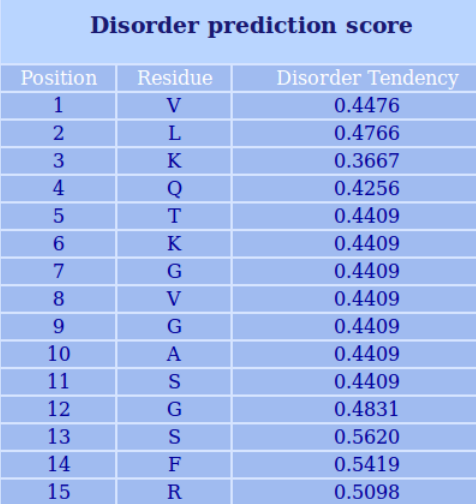
\includegraphics[width=0.5\textwidth]{img/iupredTabla.png} 
\caption{}
\label{iupredResults}
\end{figure}

% \begin{figure}[h!]
% \centering
% \begin{subfigure}[ht]{\linewidth}
% \centering
% 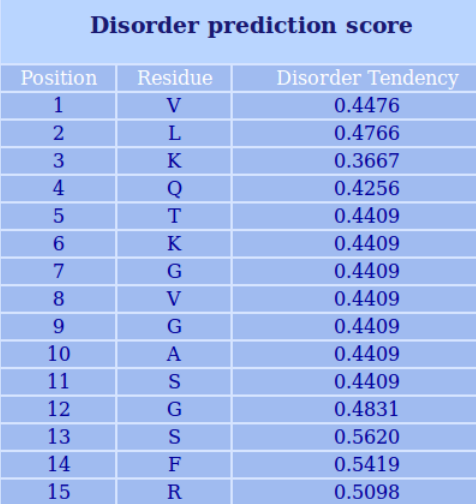
\includegraphics[width=0.5\textwidth]{img/iupredTabla.png} 
% \caption{}
% \label{iupredTabla}
% \end{subfigure}
% 
% \begin{subfigure}[ht]{\linewidth}
% \centering
% 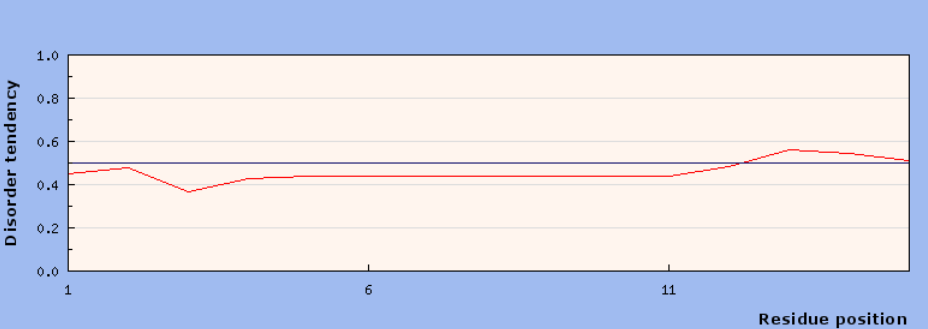
\includegraphics[width=0.7\textwidth]{img/iupredGrafico.png} 
% % 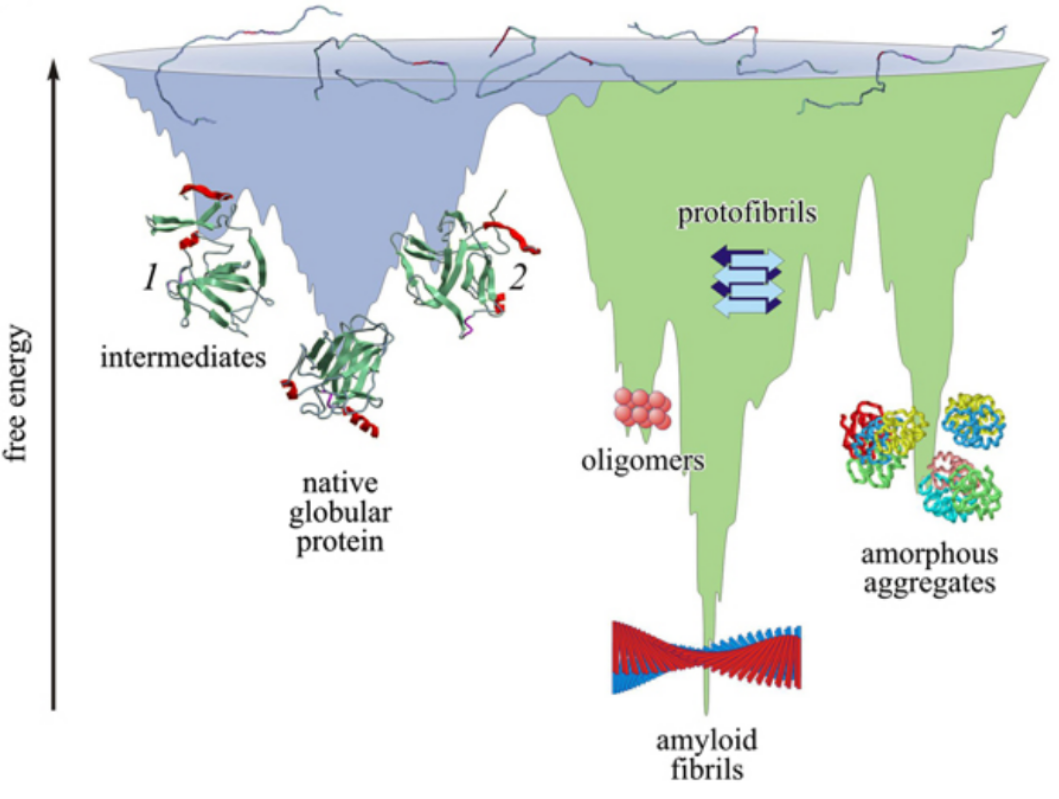
\includegraphics[width=0.7\textwidth]{img/globularEnLandscape.png} 
% \caption{}
% \label{iupredGrafico}
% \end{subfigure}
% 
% \caption{}
% \label{iupredResults}
% \end{figure}


Utilizando nuestro esquema de evaluación, estos valores resultan en los siguientes puntajes:

\vspace{0.5cm}
\begin{tabular}{lllllllllllllllll} 
\hline
Secuencia & \textbf{V} & \textbf{L} & \textbf{K} & \textbf{Q} & \textbf{T} & \textbf{K} & \textbf{G} & \textbf{V} & \textbf{G} & \textbf{A} & \textbf{S} & \textbf{G} & \textbf{S} & \textbf{F} & \textbf{R} \\ \hline
Evaluación con IUPred & 1 & 1 & 1 & 1 & 1 & 1 & 1 & 1 & 1 & 1 & 1 & 1 & 0 & 0 & 0\\ \hline
\end{tabular}







% 
% 
% 
% 
% 
% % RESUMEN SACADO DEL REVIEW
% % 
% % Dosztanyi et al. suggested that a large number of interresidue interactions is responsible for structure stabilization of proteins [50, 51]. In contrast, IDPs don’t have sufficient numbers of stabilizing inter-residue interac-
% % tions. Based on this reasoning, an IUPred algorithm estimating the inter-residue interactions was designed. First, the interaction energy between each pair of amino acids
% % based on their C β positions was estimated. This was done by calculating the potential mutual contact energies for
% % all amino acid pairs in a dataset of globular proteins with known structure. This is a fairly standard approach in
% % computational biology, and in this work Dosztanyi et al. compared several such mutual contact energies estimated
% % previously by other researchers, with the set developed by Thomas and Dill, found to be the best in this particu-
% % lar application [92]. The various pairwise energies were assembled into a 20x20 energy matrix, which was used
% % in the next step, the estimation of the mutual interaction energies for any given protein. The prediction utilizes
% % this energy prediction matrix and the amino acid compositions put into a quadratic expression. These statistical values represent the ability to form stabilization contacts
% % between amino acids in polypeptide chains. The potential mutual interactions were estimated using amino acid
% % compositions, not three-dimensional structures. These composition-based energies were compared with three-
% % dimensional structure-based energies of the proteins for which the actual side chain interactions are known. The
% % composition-based potential mutual interaction energies and the structure-based energies were found to be highly
% % correlated, thus the former can be used to estimate the latter even when the structures are not known. To use
% % this approach to predict structure or disorder, composition-based calculations for a set of proteins that fold
% % into three-dimensional structures were compared with composition-based calculations for a set of disordered
% % proteins. The estimated potential interaction energies for the structured proteins were much greater than the same
% % energies for the unstructured proteins, and from these results the energy boundary between ordered and disor-
% % dered proteins as a function of length was determined. This boundary allows the recognition of intrinsic disor-
% % der. In brief, if a sequence contains too few hydrophobic residues, then the composition-based potential mutual in-
% % teraction energy will necessarily be too small and thereby indicate the lack of potential for folding
% 



% Partiendo del concepto general que la conformación nativa está determinada por la estructura primaria de la proteína, y que esta conformación se corresponde con el mínimo global del
% espacio conformacional, es posible parametrizar un modelo que permita predecir este mínimo de energía sin asumir ninguna conformación estructural. (Ref. 2)
% Esta aproximación es posible ya que la contribución energética de un residuo depende, no solo del tipo de aminoácido, sino también de los potenciales parejas de interacción en la secuencia. 
% El aporte de un residuo será más favorable si la secuencia en la que se encuentra contiene más residuos que pueden formar interacciones favorables con este. 
% La forma de plantear este modelo es mediante una expresión cuadrática sobre la composición de aminoácidos de la secuencia:
% Los valores de n representan las frecuencias de aminoácidos i y j en la secuencia.
% El valor de P es el parámetro a estimar, el cual se deriva a partir del modelo mencionado previamente, que evalúa la energía a partir de las interacciones que ocurren en la estructura. 
% El ajuste se realiza minimizando la diferencia entre ambas ecuaciones.
% De esta forma, mediante un ajuste de mínimos cuadrados se puede parametrizar el modelo a partir de datos de estructuras pertenecientes a proteínas globulares.
% Dado que las proteínas globulares forman un gran número de interacciones entre los residuos (lo que les provee la energía estabilizante para superar la pérdida de entropía), 
% y las proteínas IU/desordenadas tienen secuencias especiales que no poseen esta capacidad de formación de interacciones, la estimación del potencial de interacción permite diferenciar entre 
% regiones de proteínas ordenadas y desordenadas. Esto transforma el modelo de predicción en un eficiente método para diferenciar secciones desordenadas de secciones con estructura definida.
% 
% Como se mencionó previamente, la parametrización de este modelo se realiza a partir de estructuras contenidas en una base de datos de proteínas globulares, 
% por lo que son datos suficientes para realizar una buena parametrización, además de ser consistentes y curadas. Esto diferencia el método de otros, que se basan en adaptar 
% un modelo a datos de estructuras correspondientes a proteínas intrínsecamente desordenadas, agrupados en bases de datos chicas, con datos obtenidos usando diversas técnicas 
% y con distintos significados del término desordenado.
%   

%   

  
  
  
  
  
  
\subsection{TMHMM: Secuencias transmembrana} \label{tmhmm}
% \cite{sonnhammer1998hidden}
% \cite{krogh2001predicting}




 
 
 
\subsection{ANCHOR: predicción de MoREs} \label{anchor}

La herramienta ANCHOR\cite{meszaros2009prediction} reutiliza el modelo definido para implementar la herramienta IUPred(ver sección \ref{iupred}), en la cual se lograba estimar la energía asociada a cada posición basándose en 
el tipo de aminoácido y la composición del contexto más próximo. Usando esta modelo, se pueden recalcular las energías de cada posición pero ``simulando'' un contexto de unión con otra proteína hipotética, lo que permite
identificar cuales son las posiciones que experimentan cambios relevantes en su energía. 

% The goal of the present work was to recognize a special class of
% disordered segments from the amino acid sequence, namely those
% that are capable of undergoing a disorder-to-order transition upon
% binding to a globular protein partner
Dado que el método busca identificar una clase especial de segmentos desordenados que son capaces de experimentar un proceso de \textit{binding \& folding}   , 
se identifican las siguientes propiedades que los segmentos buscados deben cumplir:
% Para esto se plantea, en primer lugar, un conjunto de propiedades que debe cumplir el segmento a identificar:
\begin{enumerate}
 \item El residuo debe pertenecer a una región larga desordenada, es decir, fuera de cualquier dominio globular.
 \item En el estado aislado, el residuo no debe ser capaz de formar uniones favorables con sus vecinos cercanos que le permitan plegarse.
%  (sin unirse a ninguna molécula), asegurándose que el residuo no es capaz de formar uniones suficientemente favorables con sus vecinos cercanos como para plegarse por sí mismo.
 \item El residuo tiene una ganancia neta de energía proveniente de la interacción con proteínas globulares.
%  El tercer criterio tiene en cuenta la capacidad del residuo para interaccionar con proteínas globulares durante la unión a éstas. 
 \end{enumerate}

Cada uno de estos criterios está asociado a un valor numérico y la predicción de los segmentos buscados se basa en una combinación lineal derivada directamente de estos.
% tres criterio, reutilizando los conceptos y parámetros definidos para la herramienta IUPred.
La ecuación asociada tendrá entonces 3 componentes que se combinan linealmente:
\begin{enumerate}
 \item El primer componente resulta de promediar los valores de \textit{score} obtenidos directamente de IUPred, en una ventana de tamaño $w1$(que deberá definirse como parte de los ajustes de este predictor)  alrededor de cada residuo. 
Esto evalúa la tendencia al desorden que tiene el entorno de cada residuo, separando regiones desordenadas de posiciones puntuales que puedan tener cierta tendencia al desorden.
\begin{equation}\label{score1}
 S_k = \frac{1}{N} \sum_{j=b_{lower}}^{b_{upper}} score_j
\end{equation}

donde $N$ es el número de aminoácidos efectivamente contenidos en la ventana para obtener el promedio del residuo $k$, y $b_{lower}$ - $b_{upper}$ los límites de esta.

\item El segundo componente evalúa la ganancia de energía que tendrá el residuo al formar interacciones de a pares con los vecinos contenidos dentro de una ventana de tamaño $w_2$. 
La ecuación asociada es idéntica a la obtenida para IUPred (ecuación \ref{modelofinal}), pero el valor de la ventana se redefine como parámetro, el valor del cual será ajustado 
al nuevo predictor de segmentos ANCHOR.
% \begin{equation}\label{score2}
% ddd 
% \end{equation}

\item El tercer componente evalúa la ganancia de energía que tendrá el residuo al formar interacciones de a pares con una proteína globular, 
con respecto a la formación de contactos únicamente entre los vecinos(componente 2). Para hacer esta evaluación, se reutiliza el modelo de IUPred, pero ahora, 
la composición del contexto con el cual se dan las interacciones estará dado por la composición de una proteína globular hipotética. 
Para esto se utiliza la frecuencia de aminoácidos estándar en estas proteínas.
La diferencia resultante entre la interacción con los vecinos propios de la secuencia y este nuevo valor calculado será:
\begin{equation}\label{score3}
E_i^{ganancia,k} = E_i^{intra,k} - E_i^{globular,k}
\end{equation}

donde $E_i^{intra,k}$ y $E_i^{globular,k}$ se calculan usando nuevamente la ecuación \ref{modelofinal}, usando las frecuencias del contexto de la posición $k$ y las frecuencias estándar, respectivamente.
\end{enumerate}

La ecuación para cada posición $k$ de la secuencia, resultante de la combinación de criterios es:
\begin{equation}\label{scorefinal}
I_k = p_1S_k + p_2E_i^{intra,k} + E_i^{ganancia,k}
\end{equation}


Varios de los parámetros de este nuevo modelo ya fueron determinados previamente utilizando datos conocidos de estructuras de proteínas globulares(durante el desarrollo de IUPred).
Queda determinar cuál es el peso de cada uno en el valor total(coeficientes de la combinación lineal) y los tamaños de la ventanas ($w_1$ y $w2$, correspondientes a los componentes 1 y 2).
% (cantidad de vecinos) que se tienen en cuenta para hacer el promedio en el componente 1 (w1).
% Valor de la ventana que se tiene en cuenta para evaluar cada el componente 2 (w2).

Para determinar los valores óptimos de estos parámetros se utilizaron dos conjuntos de datos: un conjunto negativo compuesto por cadenas de proteínas globulares y un conjunto de resultados positivos compuesto por complejos formados por segmentos desordenados unidos a proteinas globulares..
% Este último conjunto de datos, representa una seria limitación ya que la cantidad de elementos que se conocen es muy limitada. 
% Dada esta condición, se considera que una ventaja de este método el reducido número de parámetros(5 en total) que se deben evaluar en base a este conjunto de datos.
Cabe destacar que no es posible entrenar el predictor utilizando un conjunto de proteínas desordenadas que se sepa que no forman uniones con proteínas globulares, 
principalmente porque no existe método preciso para comprobar que esto NO ocurre. 
A pesar de esta condición, y que la cantidad de datos del conjunto de resultados positivos es considerablemente limitada, una ventaja del método es que contiene sólo 5 parámetros para los cuales se deben evaluar sus valores óptimos. 

% Dado que el resultado de ANCHOR es una combinación de varios aportes, principalmente la tendencia al desorden y la sensibilidad al estar en un entorno estructurado, 
% el resultado obtenido es relativamente independiente del score obtenido únicamente con IUPred. 

Como se define en \cite{dosztanyi2009anchor},las regiones que tienen un $score>0.5$ se puede tomar como potneciales segmentos de unión.
Dentro de nuestro esquema de evaluación, los segmentos de unión representan posibles pérdidas de flexiblidad en la región linker y, por lo tanto, se toman como propiedades negativas.
De esta forma, los residuos que posean $score>0.5$ tendrán un puntaje asociado = 1 como resultado de la evaluación.
% la herramienta ANCHOR se aplica utilizando un punto de corte igual a 0.5, como se define en el servidor . 
% Los residuos de la secuencia que tengan un valor asociado mayor a éste se considerarán como posiblemente pertenecientes a segmentos desordenados de unión a proteínas.   

Por ejemplo, la evaluación de la secuencia \texttt{TFSLWKPENMLSPDD} con ANCHOR devuelve los valores de \textit{score} mostrados en la figura \ref{anchorResults}. 

\begin{figure}[ht]
% {\linewidth}
\centering
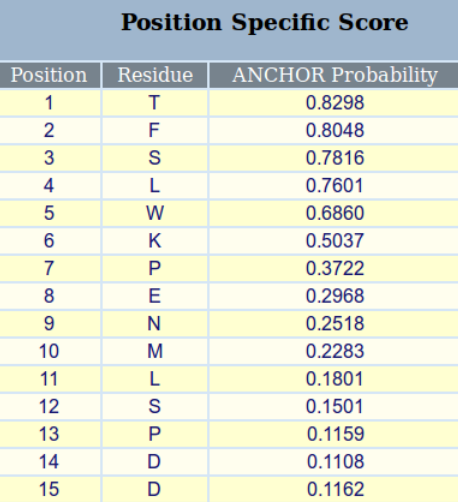
\includegraphics[width=0.5\textwidth]{img/anchorTabla.png} 
\caption{}
\label{anchorResults}
\end{figure}

Las posiciones 1-6 tienen asociados valores $>0.5$. Aplicando nuestro esquema de evaluación, estos resultados se traducen en la siguiente tabla de puntajes:

\vspace{0.5cm}
\noindent
\begin{tabular}{llllllllllllllll} 
\hline      
Secuencia & \textbf{T} & \textbf{F} & \textbf{S} & \textbf{L} & \textbf{W} & \textbf{K} & \textbf{P} & \textbf{E} & \textbf{N} & \textbf{M} & \textbf{L} & \textbf{S} & \textbf{P} & \textbf{D} & \textbf{D} \\ \hline
Evaluación con ANCHOR & 1 & 1 & 1 & 1 & 1 & 1 & 0 & 0 & 0 & 0 & 0 & 0 & 0 & 0 & 0\\ \hline
\end{tabular}





\subsection{Limbo: Interacción con chaperonas} \label{limbo}

El algoritmo Limbo\cite{van2009accurate} es un predictor de sitios de unión a la chaperona DnaK, representante de la extensa familia Hsp70, que se especializa en la unión de regiones hidrofóbicas expuestas, generalmente
presentes en polipéptidos desplegados. El método se desarrolló utilizando una combinación de información secuencial y estructural para analizar el perfil de secuencias que se unen a esta chaperona.

El primer paso en el desarrollo del método es crear un predictor basado exclusivamente en información secuencial.
Para armar el set de aprendizaje que se usará para esto, se realizaron una serie de ensayos experimentales de unión a péptidos, los cuales se inmobilizaron unidos a una membrana de celulosa, 
y luego de la incubación con DnaK se detectó la unión mediante un anticuerpo específico.

Los pépetidos usados en los ensayos de unión se obtienen de 3 conjuntos distintos. Un primer set se obtiene de predicciones basadas en el uso de Tango, asumiendo que la DnaK se une a secuencias propensas a formar agregados.
Usando los resultados obtenidos con el primer set, se desarrolla un predictor simple de unión a DnaK, utilizado para la búsqueda de sitios en el proteoma de E.coli 
y separando las proteínas cortas con al menos dos de estos sitios de unión, las cuales conforman el set 2. El último conjunto corresponde a dos péptidos supuestamente reconocidos por la DnaK, ubicados en el factor$\sigma$ de la RNA-polimerasa.

Los resultados de los ensayos fueron filtrados para separar aquellos que resultaban en señal positiva aún cuando no se realizaba el paso de incubación con DnaK (falsos positivos). 
La señal de todo el conjunto resultante se corrigió usando esta señal de control negativo. Finalmente los resultados se dividieron, según dos valores de cutoff(alto y bajo), para dar 2 conjuntos de péptidos:
los que son reconocidos por la DnaK y lo que no. El set de aprendizaje final se construye obteniendo primero todas las subsecuencias de 7 residuos posibles. 

Del set de péptidos de no-unión todos los posibles heptapéptidos formados son seleccionados, 
mientras que del set de péptidos de unión positiva sólo se incluyen aquellos que dan una mayor energía de unión a DnaK(evaluada mediante el campo de fuerzas de FoldX).
A partir de los conjuntos de heptapéptidos positivos y negativos se obtienen dos matrices PSSM y una matriz final se obtiene restando los valores de score de la PSSM de no-unión a los valores encontrados en la PSSM positiva.

De manera independiente se contruyó un perfil secuencial a partir de un análisis puramente estructural de unión a DnaK.
Para esto se hizo primero un análisis de mutaciones posicionales sobre el heptapéptido unido a la DnaK utilizando la estructura de ésta(cristalizada junto con un hepapéptido) y el campo de fuerzas FoldX. 
En primer lugar se mutaron todas las posiciones a Alanina y luego cada posición fue mutada individualmente a cada uno de los restantes 19 aminoácidos.
Se obtuvieron asi los valores de $\Delta\Delta$G para cada residuo y cada posición. 
The more
negative the DDG, the better the residue fits DnaK binding. To
convert each DDG into a PSSM score, we took the negative of
each DDG and filled the structure-based PSSM accordingly.


Los valores de todas las matrices son optimizados mediante un algoritmo de validación cruzada el cual permite eliminar algunos péptidos de los conjuntos de aprendizaje .
Los perfiles resultantes, representados en las PSSMs obtenidas del análisis secuencial y del análisis estructural se combinan para dar el predictor final. 

La versión final de la matriz y un script implementado en Python para realizar el análisis fue provisto por los desarrolladores del método.
El valor de \textit{threshold} utilizado es 11.08(valor por default). Para utilizar el método de manera local se corre el script provisto y se pasa por parámetro el archivo conteniendo las secuencias a analizar en formato fasta.
El resultado contiene una lista de heptapéptidos cuyo score calculado supera el valor del \textit{threshold}.
Por ejemplo, analizando la secuencia \texttt{DLWKLLPENNVLSP}, el resultado obtenido es:

\noindent
\texttt{1 DLWKLLP 11.7190683353}   \\
\texttt{3 WKLLPEN 23.0607028837} 

Este resultado indica que los heptapéptidos DLWKLLP y el WKLLPEN, poseen valores de score superior al \textit{threshold}(11.7190683353 y 23.0607028837, respectivamente).
Utilizando nuestro sistema de evaluación, se aumenta en 1 el puntaje de todas las posiciones asociadas a cada (tener en cuenta que algunas posiciones pueden sumar mas de 1 ya que los heptapéptidos pueden estar solapados).
A partir de los resultados anteriores, el puntaje de la evaluación es:

\vspace{0.5cm}
\noindent
\begin{tabular}{llllllllllllllll} 
\hline      		
Secuencia & \textbf{D} & \textbf{L} & \textbf{W} & \textbf{K} & \textbf{L} & \textbf{L} & \textbf{P} & \textbf{E} & \textbf{N} & \textbf{N} & \textbf{V} & \textbf{L} & \textbf{S} & \textbf{P} \\ \hline
Evaluación con Limbo & 1 & 1 & 2 & 2 & 2 & 2 & 2 & 1 & 1 & 0 & 0 & 0 & 0 & 0 \\ \hline
\end{tabular}







% Para desarrollar el algoritmo predictor, lo que se realizó fue:
% 
% ARMAN 3 GRUPOS DE PEPTIDOS (ver de donde salen los 3 grupos)
% PRUEBAN TODOS LOS PEPTIDOS MEDIANTE ENSAYO DE UNION A DnaK: sintetizan los peptidos unidos a placa de celulosa, los lavan, los incuban con DnaK y los revelan con un anticuerpo anti-DnaK. 
% (hacen ademas controles negativos de donde vuelan un par de peptidos que se unen directamente al anticuerpo, ademas restan el valor de fluorecencia que aparece cuando no ponen peptidos)
% Del total de peptidos se dividieron en conjuntos de peptidos binders y peptidos no binders(usando dos valores de cutoff - un valor alto y un bajo). 
% De cada uno de estos conjuntos se separo un pequeño % como conjunto de prueba(para probar luego que tal funciona el predictor que se va a hacer) y un gran % es el que luego se usa para el set de aprendizaje? (conjunto benchmark)
% Para poder armar una matriz de score especifica de posicion(PSSM) es necesario que todos los peptidos del conjunto de aprendizaje tengan la misma longitud. El conjunto de aprendizaje en si se obtiene dividiendo los peptidos binders y los no binders en heptapéptidos. Para el conjunto de no binders se tomaron todas las posibles subsecuencias de longitud 7 como negativos(y se agregaron al conjunto negativo de aprendizaje). Para el conjunto de binders no es tan simple, entonces se utilizo el campo de fuerzas FoldX: se evaluo la energia de union para cada heptapeptido posible(subsecuencias) y se agrega al conjunto de aprendizaje el mejor heptapeptido.(tambien se agregaron aquellos que tenian una enegia de union en un rango de 0.5kcal/mol menor)
% Construccion de la PSSM basada en datos de secuencias: inicialmente se construyeron 2 PSSMs separadas basandose en los conjuntos de aprendizaje positivos y negativos. La frecuencia observada se calculo normalizando el numero de ocurrencias de un dado residuo por el numero de secuencias totales en el conjunto de aprendizaje. La frecuencia esperada es la ocurrencia de residuos obtenida de la base de datos SwissProt. El valor que se usa en la PSSM resultante es el logaritmo de la relacion entre la frecuencia observada y la frecuencia esperada. Se generaron asi una PSSM que representa el perfil de secuencia favorable para la union a DnaK(obtenida a partir del conjunto de binders) y otra PSSM que representa el perfil desfavorable(obtenida a partir del conjunto no binder). Estos datos se integran en una misma PSSM cuyos valores estan dados por la resta de ambos valores(valor binder - valor no binder).
% Construccion de la PSSM basada en datos estructurales: se uso como template la estructura cristalizada de DnaK, junto con la cual estaba co-cristalizado un peptido con la secuencia NRLLLTG, el cual muestra el motivo(estructural?) reconocido por la DnaK, constituido por un minimo de 7 residuos en una conformacion extendida. 
% Para conocer el aporte energetico de cada posible residuo en cada una de las 7
% posiciones se utilizo nuevamente FoldX para hacer un scan posicion por posicion.
% En primer lugar se pusieron todas alaninas. Después se fueron mutando cada
% posicion por los 19 residuos restantes. Para cada uno se calcula el valor de la 
% diferencia energética con el valor del de alanina $\Delta\Delta$G (cuanto mas negativo es este 
% valor mejor es el binding). El valor que se usó para llenar la PSSM es el negativo de 
% este valor $\Delta\Delta$G.
% Dado que los valores se evaluaron mutando las posiciones sobre un backbone fijo,
% este backbone va a influenciar la PSSM resultante. Lo que se hizo entonces fue
% generar distintas PSSMs utilizando múltiples conformaciones de backbones de 
% toda la estructura de la DnaK, obtenidas de un ensamble de conformaciones 
% resueltas por NMR (para cada una se hizo una PSSM y se hizo la evaluación de 
% la ROC). Los resultados de las estructuras del ensamble NMR fueron mucho peores
% que el de la estructura cristalizada y resuelta por rayos X, por lo tanto se uso esta
% solamente
% 
% 
% La evaluación de la performance se hizo mediante 3? tests que se aplican sobre las dos PSSM: la PSSM basada solo en información secuencial y los mismos tests sobre la PSSM que combina información secuencial y estructural. Los tests consisten en calcular el MCC para la evaluación del set de entrenamiento, calcular el MCC mediante una cross-validation(se separan distintos grupos -***EN BASE A QUE???** del set de entrenamiento inicial y se generan nuevos PSSM en base a esto y evaluándolo sobre el resto del conjunto. Se calcula el MCC para cada combinación de grupos y se saca el valor medio), el otro test es calcular el MCC resultante de evaluar contra el conjunto independiente(separado al principio) para la PSSM entrenada con todo el conjunto de pruebas.
% El resultado da que las 2 primeras pruebas son un poquito mejores para la PSSM hecha solo en base a secuencias, pero en la prueba sobre el conjunto independiente la PSSM basada solo en secuencias da muy mal y la PSSM con informacion secuencial es considerablemente mejor. Esto indicaría que la informacion estructural ayuda a hacer el predictor mas general.
% 
% 
% % *****************************************************
% % FALTA DESDE DONDE DICE:  Although the heptapeptides in the learning sets were selected on a methodologically acceptable basis, inconsistencies in the learning set selection could not be excluded.
% 












\subsection{Formación de agregados}
\label{agregados}


% En el capítulo 1 vimos las propiedades más importantes de los agregados formados por proteínas.


La formación de agregados amorfos y de fibrillas amiloides son procesos diferentes, sin embargo comparten ciertas características similares ya que ambos están asociados con el enriquecimiento de estructuras de hojas-$\beta$ 
en la forma agregada, por lo que en gran medida pueden analizarse de forma conjunta.

Como se vió, la estructura de las fibrillas amiloides es altamente estructurada y por lo tanto las preferencias de aminoácidos serán mucho más específicas en relación a la posición comparado con la formación de agregados amorfos.
La formación de estos agregados amorfos es mucho menos dependiente de los residuos en cada posición y, por lo tanto, su tendencia puede predecirse si se evaluan los parámetros biofísicos generales sobre la comppsición, sin necesidad de 
evaluar propiedades específicas de secuencia.
% y, en principio, cualquier secuencia que adopte una conformación extendida, no tenga grupos  y sea suficientemente hidrofóbica 
% puede agregarse para dar esta conformación
% Amorphous $\beta$-sheet aggregation, however, is less position-dependent and can, in principle, be achieved by any sequence that can adopt an extended conformation, 
% is sufficiently hydrophobic and has no unsatisfied hydrogens or electostatic groups. 
% POR QUE NO USAMOS UN PREDICTOR ESPECIFICO??


% METODS DISPONIBLES PARA HACER LA DETECCION
En \cite{hamodrakas2011protein,redler2014computational,agrawal2011aggregation} se describen y evaluan una gran cantidad de software/metodos existentes para predecir agregacion desestructurada y formación de fibras amiloides, 
Cada método hace sus propias hipótesis e implementa predictores independientes, los cuales varían desde análisis muy simples (por ej. análisis de la composición secuencial) a métodos específicos más complejos.
La capacidad para formar hojas-$beta$ es una característica central de las evaluaciones ya que es un denominador común de la formación de agregados.




En primer lugar evaluaremos la tendencia a formar agregados utilizando TANGO(ver sección \ref{tango}). 
Este método se basa en el uso de principios fisicoquímicos que gobiernan la formacion de hojas-$\beta$
% extended by the assumption that the core regions of an aggregate are fully buried
, de manera que el método no es específico para la formación de agregados amorfos o amiloides.
% Like all algorithms that use averaged physicochemical properties to detect aggregation hot spots, TANGO is not specific for amyloid formation or amorphous beta-aggregation. 



% En cuanto a los agregados amiloides específicamente, 
En la introduccion se plantearon algunas propiedades fisicoquimicas simples con respecto a la composición de secuencias con tendencia a formar estas estructuras agregados amiloides específicamente.
En particular, las características mas importantes son la alta hidrofobicidad y baja carga neta, además de tendencia intrinseca a adoptar conformaciones de hoja-$\beta$ en su estructura primaria.
Se cree que las regiones propensas a formar agregados(APRs como se vió previamente) son segmentos con estas características que normalmente se encuentran ocultos en el núcleo hidrofóbico de la estructura plegada pero
bajo condiciones de reestructuración del plegamiento o cuando se adoptan estados \textit{misfolded}, estos segmentos pueden quedar expuestos al solvente e iniciar la formación de agregados.

% \cite: The triple power of D-3: Protein intrinsic disorder in degenerative diseases
Estos conocimientos forman la base para el desarrollo de una gran variedad de aproximaciones bioinformáticas para predecir tendencias a formar agregados a partir de la secuencia primaria.
Se debe tener en cuenta, a la hora de analizar los resultados obtenidos con esto métodos, que la existencia de APRs en la secuencia es una condición necesaria pero no suficiente para la formación de agregados


Algunos métodos intentan distinguir los agregados amorfos de la formación de fibrillas amiloides. 
Sin embargo, dado que la cantidad de secuencias que generan estructuras amiloides y se han validado experimentalmente es relativamente baja, los algoritmos basados puramente en secuencia no poseen 
suficiente información como para distinguir los distintos tipos de agregados.
% They generally also have rather poor predictive capabilities toward amyloid sequences from yeast prions and functional amyloids. 
Por otro lado, los métodos que se basan en conceptos estructurales obtenidos por homología pueden, en principio, proveer predicciones más específicas aunque también están limitados por la cantidad de estructuras determinadas disponibles.

Para evaluar específicamente la formación de fibrillas amiloides utilizaremos, en primer lugar, Waltz (descrito en la sección \ref{waltz}),
el cual combina información secuencial, parámetros fisicoquímicos y aspectos estructurales que, como se dijo, pueden no funcionar muy bien de forma aislada pero permitir una predicción eficiente si se combinan.


% PASTA
PASTA es otra de las herramienta que utilizamos para evaluar la tendencia a formación de agregados amiloides. 
PASTA obtiene potenciales estadisticos para la formación de estructuras de hojas-plegadas-$\beta$ a partir de proteinas globulares y los utiliza para
predecir cuales son los segmentos de una secuencia que le proveen a la proteína la capacidad de estabilizar la estructura supramolecular cross-$\beta$ característica de las fibrillas amiloides.
% predicts which interacting portions of a given protein are stabilizing the cross-beta structure by using an energy function. 
% r las energias asociadas a distintos emparejamientos entre secuencias formando una estructura tipo fibrilla amiloide. 

Por último, en el capítulo 1 se dejó planteada la idea sobre la existencia de subsecuencias que podrían promover y guiar la agregación para dar estructuras amiloides.
En el trabajo realizado en \cite{de2004sequence} se analiza esta idea y en \ref{determinantesSecuenciales} explicamos los resultados obtenidos y como los utilizamos para la detección 
de la tendencia a formar este tipo de agregados dentro de nuestro método.





























\subsubsection{Tango}\label{tango}
% 
% El método se deriva a partir de aplicar la mecanica estadistica a un conjunto de datos experimentales obtenidos de los residuos dentro de proteinas que promueven el 'agregamiento ordenado' o la formacion de amyloids. 
% El algoritmo resultante permite identificar las regiones de agregacion beta dentro de una secuencia.
% El algoritmo tiene en cuenta un conjunto de estados(conformaciones) posibles: alfa helice, hojas beta, beta-turns, estado plegado(nativo??*****ver abajo) y agregado de hojas beta.
% Ademas, se asume incialmente que la region en el estado de agregado de hojas beta esta totalmente internalizada y tiende a satisfacer el potencial de puentes de hidrogeno. 
% El metodo TANGO tiene tambien en cuenta la estabilidad de la proteinas y los parametros fisicoquimicos tales como el pH, la concentracion, la fuerza ionica y la concentracion de trifluoroetanol.
% 
% Cada segmento de una proteina puede estar en alguno de los estados conformacionales de acuerdo con una distribucion de Boltzman. 
% Es decir, la frecuencia con la que ese segmento adopta un estado en una poblacion es relativa a su energia, la cual se deriva de consideraciones estadisticas a partir de datos empiricos.  
% Para predecir la agregado beta de un segmento, Tango calcula la funcion de particion del espacio de fases conformacionales.
% 
% 
% ****la inclusion del estado plegado dentro de la funcion de particion tiene como objetivo ayudar a predecir efectos de agregacion debido a mutaciones puntuales en proteinas que naturalmente adquiren un estado plegado. La inclusion de este estado permite ver la competencia entre este estado natural de plegado y otros estados estructurales incluidos en la particion. De esta forma se puede predecir la tendencia a la agregacion del estado desnaturalizado y tambien las mutaciones que aumentan la tendencia a la agregacion de la proteina desestabilizando el estado plegado.
% 
% 
% 
% 
% Generally speaking, it is believed that aggregation occurs when protein segments with a high hydrophobicity, a good $\beta$-
% sheet propensity and a low net charge are solvent-exposed so that they can associate, act as nuclei for $\beta$-aggregation, and
% therefore initiate the formation of an intermolecular $\beta$-sheet (21, 78-82). In the folded state, such aggregation-prone segments are
% buried, not exposed to the solvent, and therefore protein does not aggregate. On the other hand, aggregation of many globular
% proteins occurs during refolding or under conditions in which denatured or partially folded states are significantly populated, i.e.
% at high concentration or as a result of destabilizing conditions or mutations (5, 14). Based on these findings, the algorithm
% TANGO was developed to predict $\beta$-aggregating stretches in proteins, based on a statistical mechanics algorithm that considers
% the physico-chemical parameters described above and also takes into account competition between different structural
% conformations: $\beta$-trn, $\alpha$-helix, $\beta$-sheet aggregates and the folded state (83).
% This algorithm accurately predicted the aggregation
% propensity of ~250 peptides, including those derived from human disease-related proteins, such as prion protein, lysozyme and
% beta 2-microglobulin. It was even able to correctly predict pathogenic as well as protective mutations of the A$\beta$, human lysozyme
% and transthyretin, and discriminates between $\beta$-sheet propensity and aggregation. Therefore, these data clearly confirmed the
% model of intermolecular $\beta$-sheet formation as a widespread underlying mechanism of protein aggregation (83). Importantly, the
% application of TANGO also showed that the $\beta$-aggregation propensity of all-$\alpha$, all-$\beta$ and mixed $\alpha\beta$ globular proteins as well as
% membrane-associated proteins was fairly similar, suggesting that $\beta$-aggregation was not determined by hydrophobicity and $\beta$-
% sheet propensity alone (82). Importantly, it has been established that globular proteins contained almost three times as much
% aggregation nucleating regions as IDPs and that the formation of highly structured globular proteins comes at the cost of a higher
% $\beta$-aggregation propensity because both structure formation and aggregation follow very similar physico-chemical rules (82).
% 



\subsubsection{PASTA}\label{pasta}


PASTA\cite{trovato2006insight} es una herramienta que permite, principalmente, predecir cuales son las regiones de un polipéptido que permiten estabilizar la estructura conocida para las fibrillas amiloides.
Para esto, realiza un calculo de las energias de interaccion entre los distintos segmentos, asumiendo que las interacciones entre aminoácidos que llevan a la formación 
de láminas-$\beta$ en proteínas globulares es el mismo que lleva a la formación de apilamientos de hebras-$\beta$ en estructuras cross-$\beta$.
% (estructura asociada a fibras amiloides).

% En primer lugar, Pasta deriva una funcion energetica a partir de un conjunto de datos de estructuras globulares (potenciales estadisticos).
PASTA deriva un potencial estadístico para cada par de residuos, extraído de una base de datos de proteínas globulares(selección de proteínas no-redundantes y con estructuras resuletas con alta definición)

Para cada posible par de residuos $a$-$b$ se dividen las instancias encontradas en 4 categorias según los residuos estén interaccionando formando una hoja plegada-$\beta$ en forma paralela($n_{ab}^p$) o antiparalela($n_{ab}^p$), 
o si no están participando de una estructura $\beta$ y sus carbonos-$\alpha$ están a menos de $6.5$\AA ($n_{ab}^c$ contactos genéricos), o a más de $6.5$\AA ($n_{ab}^d$ , pares desordenados sin contacto). 

A partir de las frecuencias obtenidos se pueden derivar valores de energía asociados a las interacciones de a pares formando de los distintos estados, asumiendo que la base de datos analizada es un sistema en equilibrio termodinámico 
a temperatura constante para todas las proteínas.
De esta forma, la tendencia de cada par $a$-$b$ a encontrarse en un estado $x$ se relaciona con el valor de la energía mediante el factor de Boltzman $p_{ab}(x)= e^{-E_{ab}^x}$. 
Aproximando $p_{ab}(x)$ se puede despejar el obtener una estimación de la energía asociada.
Las tendencia se define como la relación entre la frecuencia observada y la esperada en el estado de referencia. Esta probabilidad esperada se puede aproximar como la frecuencia observada para todos los pares.
Utilizando los valores definidos previamente, se despeja el valor de $E_{ab}^x$ que corresponde a la diferencia en energía entre un estado $x$ y el estado que se toma como referencia.
% El método asume que la forma soluble(estado de referencia) es nativamente desestructurada, por lo que hay que tener cuidado cuando se lo usa para predecir proteinas que nativamente adquieren una estructura globular.
El valor de energía resultante para cada estado $x$ queda definido por:

\begin{equation}
{E_{ab}^x = -log\left(\dfrac{\dfrac{n_{ab}^x}{n_{ab}}} {\dfrac{\sum\limits_{ab} n_{ab}^x}{\sum\limits_{ab} n_{ab}}}\right)}
\end{equation}


% Para derivar este valor, lo que hace es ver cual es 
% la probabilidad de encontrar cierto par de residuos enfrentados en hebras vecinas dentro de una lámina-$\beta$. 
% Se extraen valores de potencial según estén interaccionando en sentido paralelo o antiparalelo.
% El valor de este potencial estadistico para cada clase(paralela,antiparalela, etc) se calcula según la relación entre la frecuencia observada y la frecuencia esperada:
% La frecuencia esperada se aproxima como: el número de pares ab (para cualquiera ab) que está en una clase dada / el número de pares ab (para cualquier ab) que hay.
% la frecuencia observada es el numero de pares ab que estan en esa clase / el total de pares ab encontrados.
% los cuales pueden ser usados 
% para calcular el valor energético para cualquier emparejamiento de dos secuencias con la misma longitud(sumando los scores de cada par que interaccione) 
El cálculo de los valores de $E_{ab}$ para los estados paralelos y antiparalelos, resulta en un par de matrices con un valor asociado(score) para cada par $a$-$b$ de residuos posibles.
Usando estos datos es posible asignar una energía total a cada emparejamiento especifico entre subsecuencias de la misma longitud, sumando los potenciales de interaccion de a pares involucrados. 
El método permite evaluar emparejamientos entre subsecuencias correspondientes a una misma o proteína o a distintas. 

Para predecir los segmentos que pueden estar involucrados en la agregación de una proteína
se prueban todos los emparejamientos posibles entre subsecuencias de ésta, en sentido paralelo y antiparalelo, y para cada uno 
se calcula la energía asociada, resultante de sumar todos los potenciales de interacción de a pares involucrados.
El método devuelve los valores predecidos en unidades PEU (PASTA Energy Units), donde 1 PEU es equivalente a aprox. 1,192 Kcal/mol 
% The server predicts aggregation in energy units where 1 PASTA Energy Unit (PEU) is equivalent to 2 KBT at room temperature, that is 1.192 Kcal/mol (see Supplementary Material). 

Lo que nosotros queremos conocer son los residuos que podrian formar conformaciones de fibra amiloide(interacciones beta) con una energia asociada
suficientemente baja, es decir, conformaciones suficientemente estables como para que esta estructura se adopte realmente en un \% considerable.
Para lograr esto debemos obviamente definir un valor de \textit{cut-off} ya que el termino ``suficientemente bajo'' es algo totalmente subjetivo. 
% El valor de cutoff se debera elegir de forma tal que se balancee la sensibilidad y la especificidad en la deteccion.
Para balancear la sensibilidad y la especificidad el método permite, entonces, modificar dos paráemtros en el análisis. En primer lugar el valor de \textit{cut-off} que se utilizará y en segundo lugar el número de emparejamientos que 
se tendrán en cuenta dentro de ese \textit{cut-off}.

Si bien la herramienta permite definir estos valores libremente, para aplicarla nos basamos en las recomendaciones analizadas en \cite{walsh2014pasta}.
En nuestro caso utilizamos el esquema de valores que se describe como más específico, utilzando un valor de \textit{cut-off}$=-5$ y teniendo en cuenta sólo el emparejamiento de menor energía aún cuando existan otros con valores menores al \textit{cut-off}. , 
Sólo usamos el primero de los emparejamientos porque, al implementar un esquema iterativo, si los emparejamientos que se encuentran por debajo  del valor de \textit{cut-off} persisten, se incrementan o se modifican,
igualmente los tendremos en cuenta a todos en las próximas iteraciones. Otra forma de implementarlo sería ``uniendo'' todos los segmentos que entran en el rango de \textit{cut-off}.
% , de forma que en cada iteración se apunte a mutar dentro de un conjunto mas amplio de segmentos. 
% En cuanto al valor definido de \textit{cut-off}, 
% e se recomienda en \cite{walsh2014pasta} es de -2.8. Cuando se agregó incorporó PASTA en la implementación de nuestra herramienta se utilizó primero este valor, el cual, en 
% un principio pareció incorporar demasiadas restricciones a la busqueda porque....... 
% Sin embargo, esto puede haberse modificado cuando se incorporaron el resto de las herramientas de evaluación. 
El \textit{cut-off} utilizado puede ser muy específico pero es sólo el punto de inicio para la incorporación de PASTA en nuestra herramienta y es uno de los parámetros que quizás sea mejor optimizar, 
buscando un valor acorde probablemente más cercano a $-2.8$ que es el próximo valor analizado en \cite{walsh2014pasta}, para tener una mayor sensibilidad. 

Una vez que se obtiene el segmento que será tenido en cuenta, simplemente se asigna un puntaje de 1 a cada posición en nuestro esquema de puntajes.
Hay que tener en cuenta que, si bien la mayoria de las veces los emparejamientos de menor energía se corresponden con emparejamientos en forma paralela e \textit{in-register} (PIRA), es decir, 
que involucre el mismo segmento en ambas moléculas que interactúan, en el caso que esto no sea así se asigna el puntaje 1 a las posiciones de ambas regiones. 

El método PASTA es ejecutado de forma local mediante un script escrito en lenguaje Perl, obtenido de sus creadores junto con las matrices de datos(energías).
Para ejemplificar el proceso de evaluación, se muestra el resultado del evaluar la secuencia \texttt{VTNVGGAVVTGVTAV}.

La ejecución de PASTA sobre esta secuencia devuelve: \\
\noindent
\texttt{pairing 0  PASTA energy -5.735704  length 13  between segments 1-13 and 1-13  parallel}

Este resultado indica que existe un emparejamiento con un score de $-5.735704$ entre dos segmentos correspondientes a la subsecuencia \texttt{VTNVGGAVVTGVT} (posiciones 1-13). 
El puntaje resultante, por lo tanto, es:

\vspace{0.5cm}
\noindent
\begin{tabular}{lllllllllllllllll} 
\hline    
Secuencia & \textbf{V} & \textbf{T} & \textbf{N} & \textbf{V} & \textbf{G} & \textbf{G} & \textbf{A} & \textbf{V} & \textbf{V} &\textbf{T} & \textbf{G} & \textbf{V} & \textbf{T} & \textbf{A} & \textbf{V} \\ \hline
Evaluación con PASTA & 1 & 1 & 1 & 1 & 1 & 1 & 1 & 1 & 1 & 1 & 1 & 1 & 1 & 0 & 0 \\ \hline
\end{tabular}





\subsubsection{Waltz}\label{waltz}

Waltz \cite{maurer2010exploring} combina información secuencial, fisicoquímica y estructural para generar una matriz específica de posición(PSSM),
en función de la cual se evalúan las secuencias para predecir la tendencia a formar agregados amiloides.

% we explored the sequence diversity of amyloid hexa-
% peptides by inspecting more than 200 peptides using various
% structural and biophysical methods,
% and used the derived data to build Waltz, a
% web-based tool that uses a position-specific scoring matrix to
% determine amyloid-forming sequences. Waltz allows users to
% identify and better distinguish between amyloid sequences
% and amorphous beta-sheet aggregates


El score para cada posición tiene, entonces, tres componentes: un componente derivado de información secuencial, un componente derivado de un conjunto de 19 propiedades fisicoquímicas, 
y un componente resultante de evaluar distintos residuos sobre un modelo estructural de la cadena carbonada de fibras amiloides.

El primer componente se obtiene a partir del análisis secuencial de una bases de datos de hexapéptidos generadores de fibrillas amiloides que han sido evaluados experimentalmente(AmylHex).
Esta base de datos y el estudio realizado están basados en hexapéptidos porque la mayoría de las secuencias amiloides disponibles hasta el momento tienen esta longitud.
De esta forma, se ha tomado como una longitud representativa del núcleo que genera la formación de amiloides, de manera que
la inserción de estos segmentos es suficiente para inducir la conversión de todo el dominio de la proteína. 

La base de datos utilizada, sin embargo, posee una alta redundancia secuencial ya que tiene una gran cantidad de entradas correspondientes a mutaciones puntuales del péptido \texttt{STVIIE}.
De esta forma, el conjunto inicial de la base de datos se utiliza para obtener una PSSM inicial e identificar nuevas instancias de hexapéptidos, los cuales fueron evaluados experimentalmente para el desarrollo de la herramienta.
A partir de este conjunto expandido de datos se realiza un alineamiento y se usa para generar una nueva PSSM, utilizando el método de puntuación por log-probabilidades(log-odd score).
Este es el primer componente de la función de scoring de Waltz.

El segundo componente se deriva de analizar un conjunto de propiedades físicas sobre el conjunto de secuencias alineadas.
Estas 19 propiedades se incluyen en la función como un score que se deriva de sumar, para cada posición y cada aminoácido, el producto entre la frecuencia de ese residuo
y el valor normalizado de la cada propiedad. De esta forma, se obtiene un perfil de las propiedades físicas para cada posición.


El último componente de la función de scoring es una PSSM derivada del modelado estructural. 
Para obtener esta matriz se utiliza el campo de fuerzas FoldX y el péptido \texttt{GNNQQNY} (proveniente de Sup35).
En primer lugar se mutan todas las posiciones a Alanina calculando el valor de $\Delta$G para obtener finalmente el hexapéptido poli-A.
Sobre este se comienzan a realizar todas las combinaciones posibles de mutaciones utilizando los 20 aminoácidos naturales, calculando ahora el valor de $\Delta$G con respecto a este hexapéptido poli-A de referencia y 
el $\Delta\Delta$G con respecto al péptido original. 
El valor del score específico para cada posición y cada aminoácido se obtiene de promediar los valores de energía fijando este aminoácido a la posición y combinando todos los demás aminoácidos posibles en el resto de las posiciones.


La función de scoring final es la combinación lineal de los tres scores detallados:

{
\large
% \centering
\begin{equation}
S_{total}= \alpha S_{secuencial} + \beta S_{propiedadesFisicas} + \gamma S_{estructural}
\end{equation}
}

Aplicando esta función, es posible obtener los valores de score asociados a un hexapéptido(la PSSM se deriva del análisis posicional de cada una de las 6 posiciones de un hexapéptido).
Para obtener los resultados de este análisis es posible utilizar un servidor web(\url{http://waltz.switchlab.org/}), el cual permite detectar todas las posiciones de una secuencia que forman parte de algun polipéptido que supera cierto
valor de \textit{cut-off}. Este valor puede ser definido por el usuario o seleccionar alguno de las opciones estándar (alta especificidad o alta sensibilidad, con valores de 97 y 79 respectivamente).

En nuestro caso obtuvimos una versión de la PSSM correspondiente al método, junto con un script en lenguaje Perl que permite detectar las posiciones que superen el \textit{cut-off} indicado.
Ejecutando el script sobre la secuencia en cada evaluación, usando un valor de \textit{cut-off} = 79 (alta sensibilidad), asignamos un puntaje igual a 1 en todas las posiciones detectadas.
Por ejemplo, ejecutando Waltz sobre la secuencia \texttt{VTNVGGAVVTGVT}, se obtiene que el segmento 6-13 forma parte de hexapéptidos con score mayor al \textit{cut-off}. Por lo tanto, el puntaje de la evaluación será:


\vspace{0.5cm}
\noindent
\begin{center}
\begin{tabular}{lllllllllllllll} 
\hline    
Secuencia & \textbf{V} & \textbf{T} & \textbf{N} & \textbf{V} & \textbf{G} & \textbf{G} & \textbf{A} & \textbf{V} & \textbf{V} &\textbf{T} & \textbf{G} & \textbf{V} & \textbf{T}  \\ \hline
Evaluación con Waltz & 0 & 0 & 0 & 0 & 0 & 1 & 1 & 1 & 1 & 1 & 1 & 1 & 1 \\ \hline
\end{tabular}
\end{center}







\subsubsection{Determinantes secuenciales de fibras amiloides}\label{determinantesSecuenciales}

El trabajo realizado en  \cite{de2004sequence} realiza un análisis secuencial en  profundidad mediante un experimento de mutagenesis a partir de un péptido amiloide diseñado \textit{de novo} en \cite{de2002novo}. 
El ensayo consiste en reemplazar sistematicamente los residuos de este péptido(STVIIE) con todos los AAs naturales, excepto Cys.

Este estudio sigue la linea de utilizar péptidos cortos para investigar elementos de la secuencia que favorecen la agregación, 
basándose en la idea que este proceso(agregación) es conducido(generado?) por fragmentos cortos de proteinas mal plegadas.

El trabajo implica la evaluación experimental de los péptidos resultantes de la mutación
El análisis revela una dependencia posicional con la formación de este tipo de estructuras de agregación, existiendo posiciones muy tolearantes y muy restrictivas a las mutaciones.
Como parte de tal trabajo, se deriva a partir de los resultados de esta mutación sistematica, un patrón secuencial que permitiría identificar tramos de secuencias formadores de fibras amiloides.

El patrón resultante es:

$\{P\}_1 -\{PKRHW\}_2 -[VLS(C)WFNQ]_3 -[ILTYWFN]_4 -[FIY]_5- \{PKRH\}_6 $

% Because the sequence space explored in this work is very small, we are conscious that many dangerous motifs cannot be detected unless a more complete pattern is provided. 
% Therefore, similar experiments on unrelated amyloid sequences would be very
% useful to refine this amyloid fingerprint.
% 
% DISCUSION DEL PATRON ENCONTRADO
% In the light of the knowledge acquired in this study, we believe that, in same way that it has been shown for globular proteins, there are general rules governing the amyloidogenicity of a polypeptide chain.
% Because a good resolution structural model of the fibrils formed by these peptides is still lacking, any discussion about the thermodynamic origin of the effect of mutation on amyloid formation would be difficult and rather speculative. Therefore, we
% have provided only a descriptive analysis of the sequential dependence found.

% EL ESTUDIO EXPERIMENTAL SE BASA EN MEDICIONES A DISTINTOS TIEMPOS(ENTRE T=0 TIEMPO=T=1mes). EN BASE A ESTO SE OBTIENE CUALES SON LAS MUTACIONES QUE MAS ACELERAN LA FORMACION DE ESTE TIPO DE FIBRAS, Y TAMBIEN CUALES MUTACIONES 
% SON LAS QUE DAN LA MAYOR FORMACION DE FIBRAS FINAL (A TIEMPO=t), LO QUE SE ENCUENTRA ES QUE ESTOS 2 EFECTOS NO SIEMPRE COINCIDEN EN LA MISMA MUTACION
% At the most tolerant positions (1, 2, and 6), one can find many substitutions that accelerate beta-sheet polymerization dramatically
% Interestingly, the more restrictive the position is, the less the number of amino acid that are capable of accelerating the process. At position 5, no substitution accelerates the process at all.
% Amino acid replacements producing abundant amyloid products are not always the substitutions that allow for a faster beta-sheet polymerization
% *************


Para validar experimentalmente el patrón, se seleccionarion algunas combinaciones de mutaciones que, de forma individual, daban altas capacidades de formación de fibras amiloides. 
% VER COMO SE HACE LA EVALUACION EXPERIMENTAL 

Este patrón fue también validado \textit{in silico}. En este análisis, se encontró que las secuencias de una base de datos que matcheaban el patron eran menos frecuentes en proteinas que las combinaciones innocuas y que, en caso de encontrarse, estaban rodeadas de aminoácidos que 
rompen esta capacidad de agregación(conocidos como amyloid breakers).


% *************

En nuestra aplicación, implementamos la búsqueda de este patrón como parte del conjunto de evaluaciones que se hacen sobre la secuencia.
El resultado de buscar la expresión regular asociada a este patron secuencial podría aportar subsecuencias que generen una tendencia a formar este tipo de fibras amiloides.

Para buscarlo lo que se hace es utilizar 




















































































\section{Elementos funcionales}


% POR QUE QUEREMOS SACAR TODAS LAS PROPIEDADES FUNCIONALES
% ¿QUE DESEAMOS PARA EL LINKER? ¿POR QUE?

El objetivo de este trabajo es lograr una herramienta que provea una secuencia capaz ser utilizada experimentalmente como linker en el proceso de ingeniería de proteínas. 
Esto implica no sólo probar con cierta certeza que tendrá la funcionalidad deseada, sino también evaluar el comportamiento en todos los pasos del proceso de ingeniería. 
Es necesario saber que las propiedades de la secuencia no afectarán este proceso de ninguna forma.
De forma general, se debe apuntar a tener una secuencia que no tenga ninguna interacción ni funcionalidad, evitando así cualquier interferencia con la expresión y utilización del producto 
de ingeniería. Esto implica que no tenga regiones target para clivaje (fosforilación, glicosilación,etc.), regiones de unión a otras proteínas, etc.
Si bien es posible reducir este análisis conociendo más detalladamente las condiciones experimentales con las que se trabajará, el objetivo de esta herramienta es que se pueda obtener 
un resultado que cumpla con el objetivo en cualquier contexto experimental. 

En este algoritmo utilizamos distintas herramientas para evaluar la estructura que adopta la secuencia, con el fin de poder llevarla hacia una composición que provea la flexibilidad
necesaria para la función de linker. 


% There are many methods, such as SMART (Simple Modular
% Architecture Research Tool) (3), PRODOM (4) , Pfam (5,6),
% PROSITE (7) and ELM (Eukaryotic Linear Motif, http://
% elm.eu.org) (8), available for finding globular domains (e.g.
% SH3, TyrKc, active sites) and linear motifs (e.g. SH3 ligands,
% LXXLL nuclear receptor ligands, tyrosine phosphorylation
% sites, post-translational modification sites) within a protein
% sequence. These methods typically rely on sequence similarity
% models, looking for recurrence of known domains or motifs by
% such means as HMMs (Hidden Markov Models) (9), pattern
% discovery
% (http://www.cs.ucr.edu/~stelo/pattern.html)
% or
% SW(Smith-Waterman)-profiles (10). Although these methods
% are of great value in annotating protein sequences, they are
% limited in their ability to uncover new features not yet
% discovered.



% Búsqueda de secuencias homólogas
% Como se desarrollo en la introducción,
las secuencias de proteinas que estan asociadas a una misma funcion tienen ciertas restricciones en su evolución, 
asociadas con funcionalidad que deben proveer y con propiedades estructurales, lo cual se da, 
principalmente, en secuencias que codifican proteinas globulares, cuyos requerimientos estructurales son mas estrictos. 
Esta restriccion en la evolucion de la secuencia resulta en una similitud secuencial entre secuencias homólogas.
Una forma de evaluar la funcionalidad asociada a una proteina, entonces, es buscando la existencia de secuencias secuencias proteicas similares en la naturaleza, que hayan sido detectadas y que se encuentren anotadas en una base de datos

Domains are now readily detectable with sequence searching programs (e.g., Blast [9] or HMMer [10]) and readily alignable by standard methods (e.g., ClustalW [11] or MUS-
CLE [12]). Known domains are now stored in a number of databases including Pfam [1], SMART [13], CDD [14] and
InterPro [15] and remain a critical component of genome annotation procedures. 

El descubrimiento de una secuencia con gran similitid y que, por lo tanto, se presume homóloga provee un primer indicio acerca de la función que está puede cumplir. 
En el contexto de la herramienta que estamos desarrollando, la información resultante de la búsqueda sirve como indicador de que posiciones puntuales son las que conforman esta similitud secuencial y que, por lo tanto, podrían inducir la función. 

Para realizar la búsqueda de similitud secuencial utilizaremos, en principio, dos herramientas:  
la herramienta BLAST (usando la base de datos SwissProt) y la herramienta PROSITE
BLAST permite hacer un overall sequence alignment frente a una base de datos de proteinas anotadas(en nuestro caso SwissProt), y por lo tanto se encontraran secuencias 

Algunas funcionalidades en las proteinas no imponen restricciones homogeneamente a lo largo de toda la secuencia y por lo tanto quizas no puedan ser detectadas por este mecanismo.
Sin embargo las secuencias asociadas a una funcion pueden tener regiones limitadas en tamaño sobre las cuales existen(se imponen) restricciones (evolutivas) muy fuertas, ya que contienen determinantes secuenciales y/o funcionales importantes.
La herramienta PROSITE contiene extracciones de estos cluster of residue types which is variously known as a pattern, motif, signature, or fingerprint. 
Usando esta herramienta se pueden buscar estos motivos en la secuencia. 

Estos motivos pueden representar funcionalidades simples que, normalmente, no representan la funcionalidad global de la proteína natural.
Sin embargo, en nuestro caso, donde estamos trabajando con secuencias artificiales, o que han sido iterativamente mutadas, 
esta herramienta nos permite detectar(principalmente en los pasos finales???) la aparición(o la existencia/que no se haya eliminado) de elementos funcionales que igualmente queremos eliminar.  









% FUNCIONALIDAD EN IDPs

% Predicting function and/or functional sites of IDPs is a task even more difficult(que predecir la conformacion desordenada). 
% Recently, significant advance has been made in this direction, based on the observation that interactions of IDPs are often mediated by short linear motifs [11]. 
% Because linear motifs are 3–15 residues in length, they contain very little sequence information and their prediction from sequence alone is fraught with very
% high false positive rates. A critical advance in this direction has been made by applying context-filters, which significantly increase prediction accuracy by taking into
% consideration motif enrichment in proteins that share the same binding partner or evolutionary history (e.g. SLiM-Finder [12]). 
% Completely different logic forms the basis of ANCHOR, which predicts disordered binding sites by estimating their interaction energy with a general partner [13], and of the molecular recognition feature predictor
% (a-MoRF-PredII  



Estas busqueda de similitud secuencial(BLAST y PROSITE) será importante en detectar dominios funcionales de distintas longitudes. 
Sin embargo, como se vio en la sección \ref{functionalLandscape}, las   
Los principales modulos funcionales encontrados en las regiones intrínsecamente desordenadas son los motivos lineales cortos (short linear motifs, o SLiMs), que se refieren a una clase de modulos de interacción compactos, 
degenerados y evolutivamente convergentes.


Encontrar los elementos funcionales conocidos en la naturaleza dentro de nuestra secuencia es, entonces, una tarea más dificil.
 
Dado que nuestro algoritmo guiara la búsqueda hacia conformaciones desordenadas, y que una propiedad característica de los LMs es su relación con un contexto de estructura desordenada\cite{fuxreiter2007local}.
será relevante para nuestro trabajo buscar este tipo de elementos con mayor detenimiento. Más aún, teniendo en cuenta las caracteristicas secuenciales de este tipo de motivos, que le 
podía esperarse que, luego de ser detectados y mutados puedan resurgir facilmente dentro de una misma ejecución, con un comportamiento similar al que ocurre en la naturaleza.




% COMO VAMOS A DETECTARLOS
Para detectar LMs se utilizará principalmente el recurso ELM, cuya aplicación en el método se describe en \ref{elm}
% DIFERENCIAS CON PROSITE
The PROSITE database has collected a number of linear protein motifs, representing them as regular expression patterns. 
PROSITE patterns have been very useful, but also suffer from severe overprediction problems and more recently the database has emphasised globular domain annotation at the expense of linear motifs.




Además de los motivos lineales, en la introducción se describieron otros modulos funcionales que pueden estar contenidos en IDRs/IDPs.
Utilizando la herramienta ANCHOR(ver \ref{anchor}) se pueden detectar motivos de reconocimiento a partir de sus propiedades estructurales lo cual, como se menciona en \ref{propiedadesConformacionales}, es importante para restringir las 
caracteristicas estructurales del peptido resultante. Sin embargo, dada su functional importance, predicting recognition elements (motifs) from sequence is of great interest, tambien para evitar la ocurrencia de funcionalidades no deseadas.
Además, el método de busqueda secuencial BLAST puede detectar, también, dominios que son fully or largely disordered or contain conserved disordered regions es decir, intrinsically disordered domains (IDDs).
Teniendo en cuenta la hipotesis desarrollada en la introduccion acerca del solapamiento entre los MoREs y SLMs, e incluso con los dominios desordenados, las herramientas utilizadas para detectar estos tres pueden proveer resultados que se solapen.
Sin embargo, como ya se describió previamente, esto no es una desventaja.


% Ademas, most protein domains that are identified using sequence-based approaches(como el utilizado en \ref{blast}) are structured, but some can be fully or largely disordered or contain conserved disordered regions,
% es decir, intrinsically disordered domains (IDDs).
% ESTO ES CORRECTO, LO SAQUE DE    \cite{tompa2009close}
% Podria entonces decir que BLAST tambien ayuda a eliminar secuencias que puuedan adoptar estructuras plegadas?? 






\subsection{ELM}\label{elm}

El recurso de motivos lineales eucariotas(ELM) \cite{puntervoll2003elm,dinkel2013eukaryotic} fue establecido con la misión de recolectar, anotar y clasificar motivos lineales cortos
(detallados en el capítulo 1 como LMs, ELMs, SLiMs o MiniMotifs). 
% The aim(del recurso) is to cover the set of functional sites that can be defined by the local peptide sequence, operating essentially independently of protein tertiary structure. 
Este recurso provee actualmente una completa base de datos con motivos conocidos validados experimentalmente, además de una herramienta 
para descubrir segmentos posiblemente correspondientes a motivos lineales sobre secuencias provistas por el usuario. 
Es relevante destacar que todos los datos anotados son curados manualmente a partir de la literatura y están a disposición de la comunidad científica.

La base de datos se organiza jerárquicamente: en el nivel superior se tiene un conjunto de tipos (actualmente hay un total de 6 tipos diferentes). 
% los tipos son: 
% 	Proteolytic cleavage sites (CLV)
% 	general ligand binding sites (LIG),
% 	sites for post-translational modification (MOD)
% 	sub-cellular targeting sites (TRG)
% 	Ligand binding classes describing docking sites (DOC): can be described as motifs that recruit a modifying enzyme using a site that is distinct from the active site
% 	destruction motifs (DEG) is a specific region of a protein sequence that directs protein polyubiquitylation and targets the protein to the proteasome for degradation
%  ESTOS ULTIMOS 2 TIPOS FUERON AGREGADOS EN EL ULTIMO TIEMPO: 
%           Technically, all docking sites and destruction motifs belong to the ‘ligand binding sites (LIG)’ type; however, grouping together motif classes of similar function adds an additional level of discrimination.

Cada tipo agrupa un conjunto de clases, y cada clase define la especificación de un dominio o familia de dominios de péptidos, 
los cuales se describen mediante una expresión regular(cadena de carácteres para describir un patrón secuencial\cite{regex}) sobre la secuencia que los compone.
Cada clase contiene al menos una instancia anotada, donde cada instancia representa una secuencia determinada experimentalmente que se ajusta a la expresión definida para la clase.
El énfasis está puesto en la validación experimental que ha sido realizada sobre estas secuencias, logrando un proceso de curación manual con las instancias que son ingresadas en la base de datos.

Dado que los motivos suelen tener solo un pequeño número de posiciones fijas, es normal que las búsquedas resulen en una gran cantidad de falsos positivos.  
Es por esto que el recurso también provee opciones para filtrar los resultados según la especie, el compartimento en el cual se va a encontrar la secuencia, etc. 
De todas formas, la validación final de la funcionalidad del motivo debe ser siempre realizada experimentalmente.

% The resource suffers from the overprediction problem inherent to small protein motifs, but we are developing context filters such as cell compartment, taxonomy and globular domain clash that can partly reduce the severity
% of the problem. 
% In this resource, we use the term ELM to denote our bioinformatical representation of a functional site including the sequence motif and its context.
% For any such analysis, the user should be aware that many matches to ELM regular expressions are false positives. 
% Before conducting experiments based on ELM results, it is strongly advisable to check if a motif match is conserved, exposed in a cell compartment in which the motif is known to be functional. 
% The ELM resource applies several filters to provide the user with such information that should ideally also be supported by the experimental evidence.


Para poder utilizar este recurso es posible hacerlo directamente a traves de la herramienta web\cite{elmweb}. 
Esta herramienta permite encontrar en una secuencia ingresada por el usuario, instancias de los motivos contenidos en la base de datos.
Otra forma de realizar esto es haciendo una búsqueda local. Para ésto es necesario descargar las expresiones correspondientes a todas las clases de la base de datos. 
A partir de estos datos, sólo queda realizar la búsqueda de la expresión regular sobre la secuencia con la que estamos trabajando.
Esta última forma es la que utilizaremos para nuestra evaluación, para lo cual utilizamos el modulo re de Python que permite buscar instancias de una expresión regular sobre una secuencia.
La base de datos utilizada corresponde a la versión 1-3-2015 obtenida de \cite{elmweb}.
% ya que nos permite independizarnos de la disponibilidad de la herramienta en el momento en que la requerimos.

La búsqueda de motivos sobre la secuencia resulta en un conjunto de subsecuencias correspondientes a cada instancia encontrada las cuales pueden estar solapadas, es decir, cada posición de la secuencia puede contener 0,1 o más instancias encontradas. 
Cada una de estas subsecuencias se trata de forma individual.
El algoritmo toma cada una de las subsecuencias resultantes y, por cada posición de éste, se suma 1 al puntaje asociado.
Se puede ver ésto en un ejemplo sencillo:
Si estamos trabajando con la secuencia PSKPLRGNAMVGL, el resultado de la búsqueda da un conjunto de 3 motivos encontrados en las subsecuencias:
% INCLUIR EXPRESIONES REGULARES, A SER POSIBLE TOMADAS DE ELM
% 
% % \vspace{0.2cm}

% \rule[-0.8\baselineskip]{0pt}{\baselineskip}
\noindent 
\begin{tabular}{c|c|c} 
% \hline
\textbf{Clase ELM} & \textbf{Expresión regular} & \textbf{Instancia(ubicación)}\\ \hline
LIG\_SH3\_2 & P..P.[KR] & PSKPLR (1-6)\\ 
LIG\_PDZ\_Class\_2 & ...[VLIFY].[ACVILF]\$ & NAMVGL (8-13)  \\
DOC\_MAPK\_1 MAPK  & [KR]\{0,2\}[KR].\{0,2\}[KR].\{2,4\}[ILVM].[ILVF] & KPLRGNAMVGL(3-13)
\end{tabular}


% \noindent 
% \begin{tabular}{lll} 
% \hline
% Clase ELM & Instancia & Descripción \\ \hline
% LIG\_SH3\_2 & PSKPLR (posiciones 1-6) &  This is the motif recognized by class II SH3 domains\\ 
% LIG\_PDZ\_Class\_2 & NAMVGL (posiciones 8-13) & The C-terminal class 2 PDZ-binding motif \\
% DOC\_MAPK\_1 MAPK  & KPLRGNAMVGL(posiciones 3-13) &interacting molecules (e.g. MAPKKs, substrates, phosphatases) carry docking motif that help to regulate specific interaction in the MAPK cascade. \\
% \end{tabular}
% The classic motif approximates (R/K)xxxx#x# where # is a hydrophobic residue.\\
% \vspace{0.4cm}
Cada instancia encontrada implica una posible funcionalidad mediada por un motivo lineal, por lo tanto, se aumenta en 1 el valor del puntaje a las posiciones involucradas \underline{para cada instancia} por separado.
El puntaje resultante de este paso es:


% \rule[-0.8\baselineskip]{0pt}{\baselineskip}
\begin{tabular}{llllllllllllll} 
\hline
Secuencia & \textbf{P} & \textbf{S} & \textbf{K} & \textbf{P} & \textbf{L} & \textbf{R} & \textbf{G} & \textbf{N} & \textbf{A} & \textbf{M} & \textbf{V} & \textbf{G} & \textbf{L} \\ \hline
LIG\_SH3\_2 (1-6) & 1 & 1 & 1 & 1 & 1 & 1 & 0 & 0 & 0 & 0 & 0 & 0 & 0\\ \hline
LIG\_PDZ\_Class\_2 (8-13) & 0 & 0 & 0 & 0 & 0 & 0 & 0 & 1 & 1 & 1 & 1 & 1 & 1 \\ \hline
DOC\_MAPK\_1 MAPK (3-13)  & 0 & 0 & 1 & 1 & 1 & 1 & 1 & 1 & 1 & 1 & 1 & 1 & 1 \\ \hline
Evaluación global ELM & 1 & 1 & 2 & 2 & 2 & 2 & 1 & 2 & 2 & 2 & 2 & 2 & 2\\ \hline
\end{tabular}

% \vspace{0.5cm}


\subsection{Prosite}

PROSITE\cite{sigrist2002prosite,prositeWeb} es un recurso que agrupa una gran cantidad de motivos secuenciales de diversas características,
lo cual permite anotar e identificar regiones conservadas en secuencias de proteínas.
De forma resumida, se puede definir como una colección anotada de motivos biológicamente significativos, dedicada a la identificación de familias y dominios de proteínas.
Esta base de datos contiene información derivada de alineamientos de múltiples secuencias homólogas. 
Los motivos resultantes se describen usando dos métodos distintos, cada uno con sus ventajas y desventajas que definen la utilidad que tendrán:

La primera forma de describir los motivos es a través de patrones secuenciales(utilizando expresiones regulares como se mostró para ELM),
en los cuales se tiene en cuenta solo la información de los residuos más significativos, descartando el resto. 
La búsqueda de un patrón en una secuencia da un resultado cualitativo: hay una coincidencia o no la hay. 
Si hay una sustitución en alguna de las posiciones de la secuencia el patrón no coincide, independientemente del tipo de sustitución que ocurrió.

Otra forma de describir los motivos es mediante perfiles(o matrices de pesos). Estos pesos proveen valores numéricos para cada posible coincidencia o sustitución cuando se busca el motivo en una secuencia. 
De esta forma, al utilizarlos en la búsqueda de un motivo, funcionan como descriptores cualitativos que consideran la similitud global en toda la longitud secuencial de un dominio o proteína. 
Un motivo puede ser encontrado en una secuencia que posee una sustitución en una posición conservada si el resto de la secuencia tiene un nivel de similitud suficientemente alto.
Estas propiedades dan una mayor sensibilidad a los perfiles con respecto a los patrones, permitiendo encontrar dominios o familias con alta divergencia que solo tienen unas pocas posiciones muy conservadas.

Un aspecto relevante de la base de datos es que, si bien se ha orientado hacia la anotación de dominios globulares por sobre motivos lineales, existen anotaciones que representan motivos lineales cortos, lo cual trae dos consecuencias. 
En primer lugar una gran cantidad de falsos positivos debido a las propiedades intrínsecas de estos y, en segundo lugar, que puede haber un solapamiento con los resultados obtenidos utilizando la herramienta ELM.

Diversas búsquedas relacionadas con patrones anotados en Prosite se pueden hacer a través de la herramienta ScanProsite\cite{de2006scanprosite,scanprositeWeb}, 
la cual permite escanear secuencias para buscar ocurrencias de los motivos, buscar motivos en una base de datos entera de secuencias, o buscar motivos propios del usuario en una secuencia.
Esta herramienta se encuentra disponible para descargar, junto con la base de datos completa de motivos secuenciales, lo que permite realizar la búsqueda de forma local.
El objetivo de nuestra herramienta es poder encontrar cualquier ocurrencia de motivos en la secuencia sobre la que estamos trabajando. 
Para esto es posible escanearla utilizando patrones y/o perfiles, y variar también los límites usados en la detección de los perfiles. 

En nuestro caso utilizaremos patrones para realizar la búsqueda, principalmente porque el tiempo de búsqueda utilizando perfiles es de aproximadamente 10 veces el que demora la búsqueda mediante patrones 
y, si bien esta diferencia es despreciable cuando se hacen búsquedas sobre una sola secuencia, al realizar evaluaciones en una gran cantidad de iteraciones la diferencia se vuelve significativa.
En segundo lugar, consideramos que la sensibilidad provista por los patrones es suficiente para los fines buscados en nuestra herramienta, al menos inicialmente.
De todas formas, es uno de los aspectos a evaluar con mayor profundidad a futuro, por lo que no se descarta extender la búsqueda para poder utilizar perfiles, al menos de forma opcional para el usuario. 
% describir si hay superposición entre elm y prosite. Se justifica usar los dos? qué hipótesis subyacente estamos usando?

Para ejemplificar el proceso de evaluación usaremos la secuencia \texttt{VKTCLALGVDINTCD}. El proceso de búsqueda usando ScanProsite identifica que contiene en su secuencia el patrón PS00008(MYRISTYL N-myristoylation site 
\url{http://prosite.expasy.org/cgi-bin/prosite/nicedoc.pl?PS00008}) ubicado en la subsecuencia \texttt{GVDINT} (posiciones 8-13), por lo tanto el puntaje correspondiente es:

\vspace{0.5cm}
\begin{tabular}{llllllllllllllll} 
\hline
Secuencia & \textbf{V} & \textbf{K} & \textbf{T} & \textbf{C} & \textbf{L} & \textbf{A} & \textbf{L} & \textbf{G} & \textbf{V} & \textbf{D} & \textbf{I} & \textbf{N} & \textbf{T} & \textbf{C} & \textbf{D}\\ \hline
Evaluación global ELM & 0 & 0 & 0 & 0 & 0 & 0 & 0 & 1 & 1 & 1 & 1 & 1 & 1 & 0 & 0 \\ \hline
\end{tabular}













\subsection{BLAST}\label{blast}
% 
% La herramienta BLAST (ref. 1 ,2 ), la cual puede ser ejecutada de dos maneras:
% 
% Una opción es a través del servidor web \cite{blastWeb}
%     Esta opción es simple pero implica ejecutar la búsqueda remotamente y retardos para obtener los resultados. 
% %     hacer una llamada al servidor remoto que ejecuta la búsqueda (http://blast.ncbi.nlm.nih.gov/). 
% %     Se puede hacer simplemente desde Python utilizando el módulo BioPython(http://biopython.org/). (http://www.biotnet.org/sites/biotnet.org/files/documents/25/biopython_blast.pdf ) 
%  
% Otra opción es instalar localmente el software para realizar la búsqueda, lo cual requiere también disponer de las bases de datos sobre las cuales se realizarán.
%     
%     (http://www.ncbi.nlm.nih.gov/books/NBK52640/).
% 
% 
% Para la implementación de nuestra herramienta se utilizará una instalación local del software BLAST junto con las bases de datos asociadas, contra las cuales se realizará la búsqueda de similitud. 
% En nuestro caso utilizaremos la base de datos UniProtKB-SwissProt \cite{bairoch2000swiss}.
% % Swiss-Prot (created in 1986) is a high quality manually annotated and non-redundant protein sequence database, which brings together experimental results, computed features and scientific conclusions. 
% % UniProtKB/Swiss-Prot is now the reviewed section of the UniProt Knowledgebase.
% 
% % (Descripción BLAST??)
% % DESCRIBIR BREVEMENTE BLAST COMO PARA UN EXPERIMENTALISTA
% % INCLUIR REFERENCIA BLAST
% % ¿QUE OPCION TOMAMOS NOSOTROS?
% % QUE SCORE TOMAMOS COMO CUTOFF?
% 
% 
% La búsqueda BLAST se basa en los cambios que pueden ocurrir entre 2 secuencias homólogas durante la evolución. 
% Las mutaciones pueden dar como resultado distintos residuos en las secuencias de proteínas, también pueden ocurrir inserciones y deleciones de residuos. 
% Cada uno de los posibles eventos tiene una frecuencia de ocurrencia asociada. El método de alineamiento utiliza un esquema de valores para asignar puntaje a cada uno de estos eventos y,  utilizando una estrategia de optimización, se exploran formas alternativas de alinear los residuos de ambas secuencias para logar sumar el máximo score.
% Realizando una búsqueda optimizada se pueden recuperar secuencias similares de una base de datos con gran cantidad de entradas, haciendo un alineamiento de la secuencia de búsqueda frente a todas las almacenadas en la base de datos. Para analizar los resultados de esta búsqueda no es posible evaluar solamente el score obtenido en cada alineamiento, sino que se debe tener en cuenta la probabilidad de que la similitud encontrada sea solo al azar. En este punto se deben aplicar métodos estadísticos para evaluar la significancia del resultado dada la longitud de la secuencia consultada y el tamaño de la base de datos.
% El resultado que devuelve la búsqueda BLAST es, en caso de éxito, un conjunto de secuencias de la base de datos ordenadas por un score de alineamiento. Además de realizar el alineamiento, BLAST provee información estadística que ayuda a descifrar la significancia biológica del alineamiento, este es el valor "expect" o e-value. Para utilizar los resultados de BLAST en nuestra herramienta utilizaremos un cutoff sobre el valor de e-value que nos de cierta certeza de que la similitud secuencial es significativa y, por lo tanto, la secuencia podría tener una función similar. El valor de cutoff utilizado es de 0.01, todas las secuencias encontradas con un e-value menor que este valor serán significativamente similares. En caso de encontrarse muchas secuencias dentro del cutoff se utilizará la primera de éstas.
% Dado que el objetivo de este paso es evaluar que posiciones tienden a una similitud con alguna secuencia natural, el resultado obtenido se utilizará para identificar estas posiciones y marcarlas para una nueva ronda de mutaciones.
% 
% % EJEMPLO DE RESULTADO
% % DESCRIBIR BIEN QUE VALORES SE OBTIENEN
% 
% Ejemplo:
% Si realizamos la búsqueda de la secuencia MVLSPADKTNVKGGWGKV, se encontrarán varias secuencias dentro del cutoff. La primer similitud es MVLSPADKTNVKAAWGKV, con un e-value de 7e-09. El alineamiento correspondiente es:
% 
% Query  1   MVLSPADKTNVKGGWGKV  18
%            MVLSPADKTNVK  WGKV
% Sbjct  1   MVLSPADKTNVKAAWGKV  18
% 
% USAR FUENTE COURIER PARA ALINEAMIENTOS
% 
% Dentro de nuestra herramienta se utiliza este resultado para marcar los posibles targets en la mutación. En el ejemplo dado, excepto las posiciones 13 y 14, todos los residuos tienen una similitud puntual con la secuencia encontrada y, por lo tanto, son targets para una próxima mutación.
% En este paso, a cada residuo que se alinea correctamente con el hit se le sumará 1 punto al valor de score asociado.
% 


























\section{Otros propiedades evaluadas}
\subsection{Carga neta de la secuencia}

% Otro de los motivos por las cuales se podría querer eliminar aminoácidos cargados es cuando se esta diseñando una proteína que se une a dna porque los residuos del linker podrían 
% entonces formar puentes salinos con los fosfatos del dna


\subsection{Absorción UV}


